\documentclass[
    a4paper,
    twoside=false
]{kaobook}

\ifxetexorluatex
	\usepackage[babelshorthands]{polyglossia}
	\setmainlanguage{russian}
    \setotherlanguage{english}
\else
	\usepackage[russian, english]{babel}
\fi
\usepackage[autostyle]{csquotes}

\usepackage{microtype}

\usepackage{kaobiblio}
\addbibresource{FormalLanguageConstrainedReachabilityLectureNotes.bib}

\usepackage[framed=true]{kaotheorems}

\usepackage{kaorefs}

\usepackage{algpseudocode}
\usepackage{algorithm}
\usepackage{algorithmicx}


\usetikzlibrary{fit,calc,automata,positioning}
\usetikzlibrary{shapes.geometric}
\usetikzlibrary{decorations.pathmorphing}

\tikzset{
    %->, % makes the edges directed
    %>=stealth’, % makes the arrow heads bold
    node distance=4cm, % specifies the minimum distance between two nodes. Change if necessary.
    %every state/.style={thick, fill=gray!10}, % sets the properties for each ’state’ node
    initial text=$ $, % sets the text that appears on the start arrow
}

\title{О достижимости с ограничениями в терминах формальных языков}
\author{Семён Григорьев}
\date{\today}

\begin{document}

\frontmatter

\maketitle
\tableofcontents

\mainmatter
\setchapterstyle{kao}

\addchap{Список авторов}

\begin{description}[style=nextline]
      \item[Семён Григорьев]
            Санкт-Петербургский государственный университет, Университетская набережная, 7/9, Санкт-Петербург, 199034, Россия \\
            \email{s.v.grigoriev@spbu.ru}\\
            JetBrains Research, Приморский проспект 68-70, здание 1, Санкт-Петербург, 197374, Россия \\
            \email{semyon.grigorev@jetbrains.com}
      \item[Екатерина Вербицкая]
            JetBrains Research, Приморский проспект 68-70, здание 1, Санкт-Петербург, 197374, Россия \\
            \email{ekaterina.verbitskaya@jetbrains.com}
      \item[Дмитрий Кутленков]
            Санкт-Петербургский государственный университет, Университетская набережная, 7/9, Санкт-Петербург, 199034, Россия \\
            \email{kutlenkov.dmitri@gmail.com}
      \item[]
\end{description}

Полный список людей, внёсших свой вклад в данную работу, можно посмотреть на страничке проекта:
\url{https://github.com/FormalLanguageConstrainedPathQuerying/FormalLanguageConstrainedReachability-LectureNotes}

\chapter*{Введение}

Теория формальных языков находит применение не только в ставших уже классическими задачах синтаксического анализа кода (языков программирования, искусственных языков) и естественных языков, но и в других областях, таких как статический анализ кода, графовые базы данных, биоинформатика, машинное обучение.

Например, в машинном обучении использование формальных грамматик позволяет передать искусственной генеративной нейронной сети, предназначенной для построения цепочек с определёнными свойствами, знания о синтаксической структуре этих цепочек, что позволяет существенно упростить процесс обучения и повысить качество результата~\sidecite{10.5555/3305381.3305582}.
Вместе с этим, развиваются подходы, позволяющие нейронным сетям наоборот извлекать синтаксическую структуру (строить дерево вывода) для входных цепочек~\sidecite{kasai-etal-2017-tag,kasai-etal-2018-end}.

В биоинформатике формальные грамматики нашли широкое применение для описания особенностей вторичной структуры геномных и белковых последовательностей~\sidecite{Dyrka2019,WJAnderson2012,zier2013rna}.
Соответствующие алгоритмы синтаксического анализа используются при создании инструментов обработки данных.

Таким образом, теория формальных языков выступает в качестве основы для многих прикладных областей, а алгоритмы синтаксического анализа применимы не только для обработки естественных языков или языков программирования.
Нас же в данной работе будет интересовать применение теории формальных языков и алгоритмов синтаксического анализа для анализа графовых баз данных и для статического анализа кода.

Одна из классических задач, связанных с анализом графов --- это поиск путей в графе.
Возможны различные формулировки этой задачи.
В некоторых случаях необходимо выяснить, существует ли путь с определёнными свойствами между двумя выбранными вершинами.
В других же ситуациях необходимо найти все пути в графе, удовлетворяющие некоторым свойствам или ограничениям.
Например, в качестве ограничений можно указать, что искомый путь должен быть простым, кратчайшим, гамильтоновым и так далее.

Один из способов задавать ограничения на пути в графе основан на использовании формальных языков.
Базовое определение языка говорит нам, что язык --- это множество слов над некоторым алфавитом.
Если рассмотреть граф, рёбра которого помечены символами из алфавита, то путь в таком графе будет задавать слово: достаточно соединить последовательно символы, лежащие на рёбрах пути.
Множество же таких путей будет задавать множество слов или язык.
Таким образом, если мы хотим найти некоторое множество путей в графе, то в качестве ограничения можно описать язык, который должно задавать это множество.
Иными словами, задача поиска путей может быть сформулирована следующим образом: необходимо найти такие пути в графе, что слова, получаемые конкатенацией меток их рёбер, принадлежат заданному языку.
Такой класс задач будем называть задачами поиска путей с ограничениям в терминах формальных языков.

Подобный класс задач часто возникает в областях, связанных с анализом граф-структурированных данных и активно исследуется~\sidecite{doi:10.1137/S0097539798337716,axelsson2011formal,10.1007/978-3-642-22321-1_24,Ward:2010:CRL:1710158.1710234,barrett2007label,doi:10.1137/S0097539798337716}.
Исследуются как классы языков, применяемых для задания ограничений, так и различные постановки задачи.

Граф-структурированные данные встречаются не только в графовых базах данных, но и при статическом анализе кода: по программе можно построить различные графы отображающие её свойства.
Скажем, граф вызовов, граф потока данных и так далее.
Оказывается, что поиск путей в специального вида графах с использованием ограничений в терминах формальных языков позволяет исследовать некоторые нетривиальные свойства программы.
Например проводить межпроцедурный анализ указателей или анализ псевдонимов (алиасов)~\sidecite{Zheng,10.1145/2001420.2001440,10.1145/2714064.2660213}, строить срезы программ~\sidecite{10.1145/193173.195287}, проводить анализ типов~\sidecite{10.1145/373243.360208}.

В данной работе представлен ряд алгоритмов для поиска путей с ограничениями в терминах формальных языков.
Основной акцент будет сделан на контекстно-свободных языках, однако будут затронуты и другие классы: регулярные, многокомпонентные контекстно-свободные (Multiple Context-Free Languages, MCFL~\sidecite{SEKI1991191}) и конъюнктивные языки.
Будет показано, что теория формальных языков и алгоритмы синтаксического анализа применимы не только для анализа языков программирования или естественных языков, а также для анализа графовых баз данных и статического анализа кода, что приводит к возникновению новых задач и переосмыслению старых.


Структура данной работы такова.
В начале (в части~\ref{chpt:GraphTheoryIntro}) мы рассмотрим основные понятия из теории графов, необходимые в данной работе. Данные разделы являются подготовительными и не обязательны к прочтению, если такие понятия как \textit{ориентированный граф} и \textit{матрица смежности} уже известны читателю. Более того, они лишь вводят определения, подразумевая, что более детальное изучение соответствующих разделов науки остается за рамками этой работы и скорее всего уже проделано читателем.
Затем, в главе~\ref{chpt:FormalLanguageTheoryIntro} мы введём основные понятия из теории формальных языков.
Далее, в главе~\ref{chpt:FLPQ} рассмотрим различные варианты постановки задачи поиска путей с ограничениями в терминах формальных языков, обсудим базовые свойства задач, её разрешимость в различных постановках и т.д..
И в итоге зафиксируем постановку, которую будем изучать далее.
После этого, в главах~\ref{chpt:CFPQ_CYK}--\ref{chpt:GLR} мы будем подробно рассматривать различные алгоритмы решения этой задачи, попутно вводя специфичные для рассматриваемого алгоритма структуры данных.
Большинство алгоритмов будут основаны на классических алгоритмах синтаксического анализа, таких как CYK или LR.
%Все главы, начиная с~\ref{chpt:GraphTheoryIntro}, снабжены списком вопросов и задач для самостоятельного решения и закрепления материала.


\begin{figure*}
  \begin{center}
    \begin{tikzpicture}[shorten >=1pt,on grid,auto]
      \node (q_linal) [text width=4cm]               {Некоторые понятия линейной алгебры};
      \node (q_graphtheory) [below of=q_linal, text width=4cm] {Некоторые сведения из теории графов};
      \node (q_fortmallang) [right of=q_graphtheory, text width=4cm] {Общие сведения теории формальных языков};
      \node (q_reglang) [below of=q_fortmallang, text width=4cm] {Регулярные языки};
      \node (q_cflang) [right of=q_reglang, text width=4cm] {Контекстно-свободные языки и грамматики};
      \node (q_mcfl) [right of=q_cflang, text width=4cm] {Многокомпонентные контекстно-свободные языки};
      \node (q_flpq) [below of=q_graphtheory, text width=4cm] {Пути с ограничениями в терминах формальных языков};

      \node (q_rpq) [below of=q_reglang, text width=4cm] {Поиск путей с регулярными ограничениями};
      \node (q_cfpq) [below of=q_cflang, text width=4cm] {Пути с ограничениями в терминах контекстно-свободных языков};
      \node (q_mcfpq) [below of=q_mcfl, text width=4cm] {Пути с ограничениями в терминах многокомпонентных контекстно-свободных языков};
      \path[->]
      (q_linal)         edge  node {} (q_graphtheory)
      (q_graphtheory)   edge  node {} (q_flpq)
      (q_fortmallang)   edge  node {} (q_flpq)
      (q_fortmallang)   edge  node {} (q_reglang)
      (q_fortmallang)   edge  node {} (q_cflang)
      (q_fortmallang)   edge  node {} (q_mcfl)
      (q_reglang)       edge  node {} (q_rpq)
      (q_cflang)        edge  node {} (q_cfpq)
      (q_mcfl)          edge  node {} (q_mcfpq)
      (q_flpq)       edge  node {} (q_rpq)
      (q_flpq)        edge  node {} (q_cfpq)
      (q_flpq)          edge  node {} (q_mcfpq)
      ;
    \end{tikzpicture}
  \end{center}
\end{figure*}

\setchapterpreamble[u]{\margintoc}
\chapter{Некоторые понятия линейной алгебры}
\label{chpt:LinAlIntro}

При изложении ряда алгоритмов будут активно использоваться некоторые понятия и инструменты линейной алгебры, такие как моноид, полукольцо или матрица.
В данном разделе необходимые понятия будут определены и приведены некоторые примеры соответствующих конструкций.
Для более глубокого изучения материала рекомендуются обратиться к соответствующим разделам алгебры.
\marginnote[*6]{
    Неообходимо понимать, что, с одной строны, в данном разделе рассматриваются самые базовые понятия, которые даются практически в любом учебнике алгебры.
    С другой же стороны, определения данных понятий оказываются весьма вариативными и часто вызывают дискуссии.
    Например, интересный анализ тонкостей определения группы можно найти в первом и втором параграфах первого раздела книги Николая Александровича Вавилова \enquote{Конкретная теория групп}~\cite{VavilovGroups}.
    Мы же дадим определения, удобные для дальнейшего изложения материала.
}

\section{Бинарные операции и их свойства}

Введём понятие \emph{бинарной операции} и рассмотрим некоторые её свойства, такие как \emph{коммутативность} и \emph{ассоциативность}.

\begin{definition}[Функция]
    \emph{Функцией} будем называть бинарное отношение на двух множествах $S$ и $T$, такое, что каждому элементу из $S$ сопоставляется ровно один элемент из $T$.
    Запись $f: S \to T$ как раз и обозначает, что функция $f$ сопоставляет элементы из $S$ элементам из $T$.
\end{definition}

\begin{definition}[Домен функции]
    Для функции $f: S \to T$, множество $S$ называется \emph{областью определения функции} или \emph{доменом функции}.
\end{definition}

\begin{definition}[Кодомен функции]
    Для функции $f: S \to T$, множество $T$ называется \emph{областью значений функции} или \emph{кодоменом функции}.
\end{definition}

\begin{definition}[Двухместная функция]
    Функцию, принимающую два аргумента, $f: R \times S \to T$ будем называть \emph{двухместной} или \emph{функцией арности два}.
    Для записи таких функций будем использовать типичную нотацию: $t = f(r, s)$.
\end{definition}

\begin{definition}[Бинарная операция]
    \emph{Бинарная операция}~--- это двухместная функция, от которой дополнительно требуется, чтобы оба аргумента и результат лежали в одном и том же множестве: $f: S \times S \to S$.
    В таком случае говорят, что бинарная операция определена на некотором множестве $S$. Для обозначения произвольной бинарной операции будем использовать символ $\circ$ и пользоваться инфиксной нотацией для записи: $s_3 = s_1 \circ s_2$.
\end{definition}

\begin{definition}[Внешняя бинарная операция]
    \emph{Внешняя бинарная операция}~--- это бинарная операция, у которой аргументы лежат в разных множествах, при этом результат~--- в одном из этих множеств.
    Иными словами $\circ: R \times S \to S$, где $R$ может не совпадать с $S$~--- внешняя бинарная операция.
\end{definition}

Необходимо помнить, что как функции, так и бинарные операции, могут быть частично определёнными (частичные функции, частичные бинарные операции).
Типичным примером частично определённой бинарной операции является деление на целых числах: она не определена, если второй аргумент равен нулю.

Бинарные операции могут обладать некоторыми дополнительными свойствами, такими как \emph{коммутативность} или \emph{ассоциативность}, позволяющими преобразовывать выражения, составленные с использованием этих операций.

\begin{definition}[Коммутативная операция]
    Бинарная операция $\circ : S \times S \to S$ называется \emph{коммутативной}, если для любых  $s_1, s_2 \in S$ верно, что  $s_1 \circ s_2 = s_2 \circ s_1$.
\end{definition}

\begin{example}
    Рассмотрим несколько примеров коммутативных и некоммутативных операций.
    \begin{itemize}
        \item Операция сложения на целых числах является коммутативной: известный ещё со школы перестановочный закон сложения.
        \item Операция умножения на целых числах является коммутативной: известный ещё со школы перестановочный закон умножения.
        \item Операция конкатенации на строках\marginnote{TODO: Здесь слова о том, что из текста далее будет понятно, почему именно точка} $\cdot$ не является коммутативной:
              \["ab" \cdot "c"  = "abc" \neq "cab" = "c" \cdot "ab".\]
        \item Операция умножения матриц (над целыми числами) $\cdot$ не является коммутативной:
              \[\begin{pmatrix}
                      1 & 1 \\
                      0 & 0
                  \end{pmatrix}
                  \cdot
                  \begin{pmatrix}
                      0 & 0 \\
                      1 & 1
                  \end{pmatrix}
                  =
                  \begin{pmatrix}
                      1 & 1 \\
                      0 & 0
                  \end{pmatrix}
                  \neq
                  \begin{pmatrix}
                      0 & 0 \\
                      1 & 1
                  \end{pmatrix}
                  =
                  \begin{pmatrix}
                      0 & 0 \\
                      1 & 1
                  \end{pmatrix}
                  \cdot
                  \begin{pmatrix}
                      1 & 1 \\
                      0 & 0
                  \end{pmatrix}
                  .\]
    \end{itemize}
\end{example}

\begin{definition}[Ассоциативная бинарная операция]
    Бинарная операция $\circ: S \times S \to S$ называется \emph{ассоциативной}, если для любых  $s_1, s_2, s_3 \in S$ верно, что  $(s_1 \circ s_2) \circ s_3 = s_1 \circ (s_2 \circ s_3)$.
    Иными словами, для ассоциативной операции результат вычислений не зависит от порядка применения операций.
\end{definition}

\begin{example} Рассмотрим несколько примеров ассоциативных и неассоциативных операций.
    \begin{itemize}
        \item Операция сложения на целых числах является ассоциативной.
        \item Операция умножения на целых числах является ассоциативной.
        \item Операция конкатенации на строках $\cdot$ является ассоциативной:
              \[("a" \cdot "b") \cdot "c"  = "a" \cdot ("b" \cdot "c") = "abc".\]
        \item Операция возведения в степень (над целыми числами) $\hat{\mkern6mu}$ не является ассоциативной:
              \[(2\hat{\mkern6mu}2)\hat{\mkern6mu}3 = 4 \hat{\mkern6mu} 3 = 64 \neq 256 = 2 \hat{\mkern6mu} 8 = 2\hat{\mkern6mu}(2\hat{\mkern6mu}3).\]
    \end{itemize}
\end{example}

\begin{definition}[Дистрибутивная бинарная операция]
    Говорят, что бинарная операция $\otimes: S \times S \to S$ является \emph{дистрибутивной} относительно бинарной операции $\oplus: S \times S \to S$, если
    \begin{enumerate}
        \item Для любых $s_1, s_2, s_3 \in S$, $s_1 \otimes (s_2 \oplus s_3) = (s_1 \otimes s_2) \oplus (s_1 \otimes s_3)$ (дистрибутивность слева).
        \item Для любых $s_1, s_2 ,s_3 \in S$, $(s_2 \oplus s_3) \otimes s_1 = (s_2 \otimes s_1) \oplus (s_3 \otimes s_1)$ (дистрибутивность справа).
    \end{enumerate}
    Если операция $\otimes$ является коммутативной, то дистрибутивность слева и справа равносильны.
\end{definition}

\begin{example}
    Рассмотрим несколько примеров дистрибутивных операций.
    \begin{itemize}
        \item Умножение целых чисел дистрибутивно относительно сложения и вычитания: классический \emph{распределительный закон}, знакомый всем со школы.
        \item Операция деления (допустим, на действительных числах) не коммутативна.
              При этом, она дистрибутивна справа относительно сложения и вычитания, но не дистрибутивна слева%
              \sidenote{
                  Здесь может быть уместно вспомнить правила сложения дробей.
                  Дроби с общим знаминателем складывать проще как раз из-за дистрибутивности справа.}.
              Так, $(a + b) / c = (a / c) + (b / c)$, но $c / (a + b) \neq (c / a) + (c / b)$.
    \end{itemize}
\end{example}

\begin{definition}[Идемпотентная бинарная операция]
    Бинарная операция $\circ: S \times S \to S$ называется \emph{идемпотентной}, если для любого  $s \in S$ верно, что  $s \circ s = s$.
\end{definition}

\begin{example}
    Рассмотрим несколько примеров идемпотентных операций.
    \begin{itemize}
        \item Операция объединения множеств $\cup$ является идемпотентной: для любого множества $S$ верно, что $S \cup S = S$.
        \item Операция сложения на целых числах не является идемпотентной.
        \item Операции \enquote{логическое и} $\land$ и \enquote{логическое или} $\lor$ являются идемпотентными.
        \item Операция \enquote{исключающее или} (\textsf{XOR}) не является идемпотентной.
    \end{itemize}
\end{example}

\begin{definition}[Нейтральный элемент]
    Пусть есть коммутативная бинарная операция $\circ$ на множестве $S$.
    Говорят, что $e \in S$ является \emph{нейтральным элементом} по операции $\circ$, если для любого $s \in S$ верно, что $e \circ s = s \circ e = s$.
    Если бинарная операция не является коммутативной, то можно определить \emph{нейтральный слева} и \emph{нейтральный справа} элементы по аналогии.
\end{definition}

\section{Полугруппа}

\begin{definition}[Полугруппа]
    Множество $S$ с заданной на нём ассоциативной бинарной операцией $\cdot: S \times S \to S$ называется \emph{полугруппой} и обозначается $(S, \cdot)$.
    Если операция $\cdot$ является коммутативной, то говорят о \emph{коммутативной полугруппе}.
\end{definition}

\begin{example}
    Приведём несколько примеров полугрупп.
    \begin{itemize}
        \item Множество положительных целых чисел с операцией сложения является коммутативной полугруппой.
        \item Множество целых чисел с операцией взятия наибольшего из двух ($\max$) является коммутативной полугруппой.
        \item Множество всех строк конечной длины без пустой строки%
              \sidenote{
                  Множество всех строк конечной длины c пустой строкой также является полугруппой.
                  Однако, такая структура является ещё и моноидом, что будет показано далее.}
              над фиксированным алфавитом $\Sigma$ с операцией конкатенации является полугруппой.
              Так как конкатенация на строках не является коммутативной операцией, то и полугруппа не является коммутативной.
    \end{itemize}
\end{example}

\section{Моноид}

\begin{definition}[Моноид]
    \emph{Моноидом} называется полугруппа с нейтральным элементом.
    Если операция является коммутативной, то можно говорить о \emph{коммутативном моноиде}.
\end{definition}

\begin{example}
    Приведём примеры моноидов, построенных на основе полугрупп из предыдущего раздела.
    \begin{itemize}
        \item Неотрицательные целые числа (или же натуральные числа с нулём) с операцией сложения являются моноидом.
              Нейтральный элемент~--- $0$.
        \item Целые числа, дополненные значением $-\infty$ (\enquote{минус бесконечность}) с операцией взятия наибольшего из двух ($\max$) являются моноидом.
              Нейтральный элемент~--- $-\infty$.
        \item Множество всех строк конечной длины с пустой строкой (строка длины 0) над фиксированным алфавитом $\Sigma$ и операцией конкатенации является моноидом.
              Нейтральный элемент~--- пустая строка.
        \item Квадратные неотрицательные матрицы%
              \sidenote{Неотрицательной называется матрица, все элементы которой не меньше нуля.} фиксированного размера с операцией умножения задают моноид.
              Нейтральный элемент~--- единичная матрица.
    \end{itemize}
\end{example}

\section{Группа}

\begin{definition}[Группа]
    Непустое%
    \sidenote{Требование непустоты здесь, как и далее, в определениях полукольца и кольца~--- дискуссионный вопрос.}
    множество $G$ с заданной на нём бинарной операцией $\circ: {G} \times {G} \to {G}$ называется \emph{группой} $(G ,\circ)$, если выполнены следующие аксиомы:
    \begin{enumerate}
        \item ассоциативность: для любых $a, b, c \in G$ выполнено $(a \circ b) \circ c = a \circ (b \circ c)$;
        \item наличие нейтрального элемента $e$: для любого $a \in G$ выполнено $e \circ a = a \circ e = a$;
        \item наличие обратного элемента: для любого $a \in G$ существует $a^{-1} \in G$, такой что $a \circ a^{-1} = a^{-1} \circ a = e$.
    \end{enumerate}
    Иными словами, группа~--- это моноид с дополнительным требованием наличия обратных элементов.
\end{definition}

\begin{definition}[Абелева группа]
    Если операция $\circ$ коммутативна, то говорят, что группа \emph{абелева}.
\end{definition}

\begin{example}
    Рассмотрим несколько примеров групп.
    \begin{itemize}
        \item Целые числа $\Z$ с операцией сложения $+$ являются группой.
              Получается дополнением моноида из предыдущего раздела обратными по сложению элементами.
        \item Целые числа $\Z$ без нуля%
              \sidenote{
                  При наличии нуля возникают трудности с нейтральным элементом.
                  Логично считать $1$ нейтральным по умножению, однако $0 \cdot 1 = 0$, а не 1, как того требует определение.}
              с операцией умножения $\cdot$ не являются группой, так как нет обратных по умножению.
              Действительно, возьмём $a = 3$, тогда должен существовать $a^{-1} \in \Z$, такой что $3 \cdot a^{-1} = 1$.
              Видим, что $a^{-1} = 1/3$, но $1/3 \notin \Z$.
        \item Множество обратимых%
              \sidenote{
                  Квадратная матрица $M$ называется обратимой, если существует матрица $N$, называемая обратной, такая что $M \cdot N = N \cdot M = I$, где $I$~--- единичная матрица.
                  К сожалению, не все матрицы являются обратимыми, потому, чтобы сконструировать группу, нам приходится требовать обратимость явно.}
              матриц с операцией матричного умножения задают группу.
    \end{itemize}
\end{example}

\section{Полукольцо}

\begin{definition}[Полукольцо]
    Непустое множество $R$ с двумя бинарными операциями $\oplus: R \times R \to R$ (часто называют сложением) и $\otimes: R \times R \to R$ (часто называют умножением) называется \emph{полукольцом}, если выполнены следующие условия.
    \begin{enumerate}
        \item $(R, \oplus)$~--- это коммутативный моноид, нейтральный элемент которого~--- $\bz$. Для любых $a, b, c \in R$:
              \begin{itemize}
                  \item $(a \oplus b) \oplus c = a \oplus (b \oplus c)$
                  \item $\bz \oplus a = a \oplus \bz = a$
                  \item $a \oplus b = b \oplus a$
              \end{itemize}
        \item $(R, \otimes)$~--- это моноид, нейтральный элемент которого~--- $\bo$. Для любых $a, b, c \in R$:
              \begin{itemize}
                  \item $(a \otimes b) \otimes c = a \otimes (b \otimes c)$
                  \item $\bo \otimes a = a \otimes \bo = a$
              \end{itemize}
        \item $\otimes$ дистрибутивно слева и справа относительно $\oplus$:
              \begin{itemize}
                  \item $a \otimes (b \oplus c) = (a \otimes b) \oplus (a \otimes c)$
                  \item $(a \oplus b) \otimes c = (a \otimes c) \oplus (b \otimes c)$
              \end{itemize}
        \item $\bz$ является \emph{аннигилятором} по умножению:
              \begin{itemize}
                  \item для любых $a \in R$ выполнено $\bz \otimes a = a \otimes \bz = \bz$
              \end{itemize}
    \end{enumerate}
    Если операция $\otimes$ коммутативна, то говорят о \emph{коммутативном полукольце}.
    Если операция $\oplus$ идемпотентна, то говорят об \emph{идемпотентном полукольце}.
\end{definition}

\begin{example}
    \label{exmpl:semiring}
    Рассмотрим пример полукольца, а заодно покажем, что левая и правая дистрибутивность могут существовать независимо для некоммутативного умножения%
    \sidenote{
        Хороший пример того, почему левую и правую дистрибутивность в случае некоммутативного умножения нужно проверять независимо (правда, для колец), приведён Николаем Александровичем Вавиловым в книге \enquote{Конкретная теория колец} на странице 6~\cite{VavilovRings}.}%
    .

    В качестве $R$ возьмём множество множеств строк конечной длины над некоторым алфавитом $\Sigma$.
    В качестве сложения возьмём теоретико-множественное объединение: $\oplus \equiv \cup$.
    Нейтральный элемент по сложению~--- это пустое множество ($\varnothing$).
    В качестве умножения возьмём конкатенацию множеств ($\otimes \equiv \odot$) и определим её следующим образом:
    \[S_1 \odot S_2 = \left\{ w_1 \cdot w_2 \mid w_1 \in S_1, w_2 \in S_2\right\},\]
    где $\cdot$~--- конкатенация строк.
    Нейтральным элементом по умножению будет являться множество из пустой строки: $\{\varepsilon\}$, где $\varepsilon$~--- обозначение для пустой строки.

    Проверим, что $(R, \cup, \odot)$ действительно полукольцо по нашему определению.
    \begin{enumerate}
        \item $(R, \cup)$~--- действительно коммутативный моноид с нейтральным элементом $\varnothing$.
              Для любых $a, b, c \in R$ по свойствам теоретико-множественного объединения верно:
              \begin{itemize}
                  \item $(a \cup b) \cup c = a \cup (b \cup c)$
                  \item $\varnothing \cup a = a \cup \varnothing = a$
                  \item $a \cup b = b \cup a$.
              \end{itemize}
        \item $(R, \odot)$~--- действительно моноид с нейтральным элементом $\{\varepsilon\}$.
              Для любых $a, b, c \in R$:
              \begin{itemize}
                  \item $(a \odot b) \odot c = a \odot (b \odot c)$ по определению $\odot$
                  \item $\{\varepsilon\} \odot a = \{\varepsilon \cdot w \mid w \in a \} = \{w \mid w \in a \} = a \odot \{\varepsilon\} = a$
              \end{itemize}
              Вообще говоря, сконструированный нами моноид не является коммутативным: легко проверить, например, что существуют непустые $a, b \in R$, $a \neq b$, $a \neq \{\varepsilon\}$, $b \neq \{\varepsilon\}$, такие что $a \cdot b \neq b \cdot a$ по причине некоммутативности конкатенации строк.
        \item $\odot$ дистрибутивно слева и справа относительно $\cup$:
              \begin{itemize}
                  \item Сначала проверим дистрибутивность слева.
                        \begin{align*}
                            a \odot (b \cup c) & = \{ w_1 \cdot w_2 \mid  w_1 \in a, w_2 \in b \cup c\}                                                \\
                                               & = \{ w_1 \cdot w_2 \mid  w_1 \in a, w_2 \in b \} \cup  \{ w_1 \cdot w_2 \mid  w_1 \in a, w_2 \in c \} \\
                                               & =  (a \odot b) \cup (a \odot c)
                        \end{align*}
                  \item Аналогично, $(a \cup b) \odot c = (a \odot c) \cup (b \odot c)$
              \end{itemize}
              При этом, в общем случае, $a \odot (b \cup c) \neq (b \cup c) \odot a$ из-за некоммутативности операции $\odot$.
              Действительно,
              \begin{gather*}
                  \{"a"\} \odot (\{"b"\} \cup \{"c"\}) = \{"a"\} \odot \{"b","c" \} = \{"ab","ac" \} \\
                  (\{"b"\} \cup \{"c"\}) \odot \{"a"\} =  \{"b", "c"\} \odot \{"a"\} = \{"ba","ca"\} \\
                  \{"ab","ac"\} \neq \{"ba","ca"\}
              \end{gather*}
        \item $\varnothing$ является \emph{аннигилятором} по умножению: для любого $a \in R$ верно, что
              $\varnothing \odot a =  \{ w_1 \cdot w_2 \mid w_1 \in \varnothing, w_2 \in a \} =  \{ w_1 \cdot w_2 \mid w_1 \in a, w_2 \in \varnothing \} = a \odot \varnothing = \varnothing$
    \end{enumerate}
\end{example}

\section{Кольцо}

\begin{definition}[Кольцо]
    Непустое множество $R$ с двумя бинарными операциями $\oplus: R \times R \to R$ (умножение) и $\otimes: R \times R \to R$ (сложение) называется \emph{кольцом}, если выполнены следующие условия.
    \begin{enumerate}
        \item $(R, \oplus)$~--- это абелева группа, нейтральный элемент которой~--- $\bz$.
              Для любых $a, b, c \in R$:
              \begin{itemize}
                  \item $(a \oplus b) \oplus c = a \oplus (b \oplus c)$
                  \item $\bz \oplus a = a \oplus \bz = a$
                  \item $a \oplus b = b \oplus a$
                  \item для любого $a \in R$ существует $-a \in  R$, такой что $a + (-a) = \bz$.
              \end{itemize}
              В последнем пункте кроется отличие от полукольца.
        \item $(R, \otimes)$~--- это моноид, нейтральный элемент которого~--- $\bo$.
              Для любых $a, b, c \in R$:
              \begin{itemize}
                  \item $(a \otimes b) \otimes c = a \otimes (b \otimes c)$
                  \item $\bo \otimes a = a \otimes \bo = a$
              \end{itemize}
        \item $\otimes$ дистрибутивно слева и справа относительно $\oplus$:
              \begin{itemize}
                  \item $a \otimes (b \oplus c) = (a \otimes b) \oplus (a \otimes c)$
                  \item $(a \oplus b) \otimes c = (a \otimes c) \oplus (b \otimes c)$
              \end{itemize}
    \end{enumerate}
\end{definition}

Заметим, что мультипликативное свойство $\bz$ (быть аннигилятором по умножению) не указыватеся явно, так как может быть выведено из остальных утверждений.
Действительно,
\begin{enumerate}
    \item $a \otimes \bz = a \otimes (\bz \oplus \bz)$, так как $\bz$~--- нейтральный по сложению, то $\bz \oplus \bz = \bz$
    \item Воспользуемся дистрибутивностью: $a \otimes (\bz \oplus \bz) = a \otimes \bz \oplus a \otimes \bz$.
          В итоге: $a \otimes \bz = a \otimes \bz \oplus a \otimes \bz$
    \item Так как у нас есть группа по сложению, то для любого $a$ существует обратный элемент $a^{-1}$, $a \oplus a^{-1} = \bz$.
          Прибавим $a^{-1} \otimes \bz$ к левой и правой части равенства%
          \sidenote{Обычно данное действие воспринимается как очевидное, но, строго говоря, оно требует аккуратного введения структур с равенством и соответствующих аксиом.}%
          , полученного на предыдущем шаге:
          \[a \otimes \bz \oplus a^{-1} \otimes \bz = a \otimes \bz \oplus a \otimes \bz \oplus a^{-1} \otimes \bz.\]
    \item Воспользуемся дистрибутивностью и ассоциативностью.
          \begin{align*}
              (a \oplus a^{-1}) \otimes \bz & = a \otimes \bz \oplus (a  \oplus a^{-1}) \otimes \bz \\
              \bz \otimes \bz               & = a \otimes \bz \oplus \bz \otimes \bz                \\
              \bz                           & = a \otimes \bz
          \end{align*}
    \item Аналогично можно доказать, что $\bz = \bz \otimes a$.
\end{enumerate}

%\section{Поле}

\section{Матрицы и вектора}

К определению матрицы мы подойдём структурно, так как в дальнейшем будем сопоставлять эту структуру с объектами различной природы, а значит определение матрицы через какой-либо из этих объектов (например через квадратичные формы) будет менее удобным.

Договоримся, что \emph{алгебраическая структура}~--- это собирательное название для объектов вида \enquote{множество с набором операций} (например, кольцо, моноид, группа и т.д.), а соответствующее множество будем назвать \emph{носителем} этой структуры.

\begin{definition}[Матрица]
    Предположим, что у нас есть некоторая алгебраическая структура с носителем $S$. Тогда \emph{матрицей} будем называть прямоугольный массив размера $n \times m$, $n > 0$, $m > 0$, заполненный элементами из $S$.

    Говорят, что $n$~--- это высота матрицы или количество строк в ней, а $m$~--- ширина матрицы или количество столбцов.
\end{definition}

При доступе к элементам матрицы используются их индексы.
При этом нумерация ведётся с левого верхнего угла, первым указывается строка, вторым~--- столбец.
В нашей работе мы будем использовать \enquote{программистскую} традицию и нумеровать строки и столбцы с нуля%
\sidenote{
    В противоположность \enquote{математической} традиции нумеровать строки и столбцы с единицы.
    Стоит, правда, отметить, что в некоторых языках программирования (например, Fortran или COBOL) жива \enquote{математическая} традиция.}%
.

\begin{example}
    Пусть есть моноид $(S, \cdot)$, где $S$~--- множество строк конечной длины над алфавитом $\{a, b, c\}$.
    Тогда можно построить, например, следующую матрицу $2 \times 3$.
    \[
        M_{2 \times 3} =
        \begin{pmatrix}
            "a"  & "ba"  & "cb" \\
            "ac" & "bab" & "b"
        \end{pmatrix}
    \]
    Для доступа к элементу матрицы будем использовать такую запись: $M_{2 \times 3}[1, 1] = "bab"$.
\end{example}

К определению вектора мы также подойдём структурно.
\begin{definition}[Вектор]
    \emph{Вектором} будем называть матрицу, хотя бы один из размеров которой равен единице.
    Если единице равна высота матрицы, то это \emph{вектор-строка}, если же единице равна ширина матрицы, то это \emph{вектор-столбец}.
\end{definition}

Операции над матрицами можно условно разделить на две группы:
\begin{itemize}
    \item \emph{структурные}~--- не зависящие от алгебраической структуры, над которой строилась матрица, и работающие только с её структурой;
    \item \emph{алгебраические}~--- определение таковых опирается на свойства алгебраической структуры, над которой построена матрица.
\end{itemize}

Примерами структурных операций является \emph{транспонирование}, \emph{взятие подматрицы} и \emph{взятие элемента по индексу}.

\marginnote{
    \begin{example}
        Транспонирование матрицы.
        \[
            \begin{pmatrix}
                "a"  & "ba"  & "cb" \\
                "ac" & "bab" & "b"
            \end{pmatrix}^\top =
            \begin{pmatrix}
                "a"  & "ac"  \\
                "ba" & "bab" \\
                "cd" & "b"
            \end{pmatrix}
        \]
    \end{example}
}
\begin{definition}[Транспонирование матрицы]
    Пусть дана матрица $M_{n \times m}$.
    Тогда результат её \emph{транспонирования}, это такая матрица $M'_{m \times n}$, что $M'[i,j] = M[j,i]$ для всех $i \in [0 : m - 1]$ и $j \in [0 : n - 1]$.

    Операцию транспонирования принято обозначать как $M^\top$.
\end{definition}

\begin{definition}[Прямая сумма матриц]
    Пусть даны матрицы $M_{n_1 \times m_1}$ и $N_{n_2 \times m_2}$.
    Тогда \emph{прямой суммой} этих матриц называется матрица $L_{(n_1 + n_2) \times (m_1 + m_2)}$ вида
    \[
        L =
        \begin{pmatrix}
            M & 0 \\
            0 & N
        \end{pmatrix}
    \]
    Где 0 обозначает нулевой блок. Прямая сумма обозначается $L = M \oplus N$.
\end{definition}

\marginnote{
    \begin{example}
        Взятие подматрицы.
        \begin{multline*}
            \begin{pmatrix}
                "a"  & "ba"  & "cb" \\
                "ac" & "bab" & "b"
            \end{pmatrix} [0 : 1, 1 : 2] = \\
            = \begin{pmatrix}
                "ba"  & "cb" \\
                "bab" & "b"
            \end{pmatrix}
        \end{multline*}
    \end{example}
}
\begin{definition}[Взятие подматрицы]
    Пусть дана матрица $M_{n\times m}$.
    Тогда $M_{n \times m}[i_0 : i_1, j_0 : j_1]$~--- это такая $M'_{(i_1 - i_0 + 1) \times (j_1 - j_0 + 1)}$, что $M'[i, j] = M[i_0 + i, j_0 + j]$ для всех $i \in [0 : i_1 - i_0 + 1]$ и $j \in [0 : j_1 - j_0 + 1]$.
\end{definition}

\marginnote{
    \begin{example}
        Взятие элемента по индексу.
        \[
            \begin{pmatrix}
                "a"  & "ba"  & "cb" \\
                "ac" & "bab" & "b"
            \end{pmatrix}[0, 1] = "ba"
        \]
    \end{example}
}
\begin{definition}[Взятие элемента по индексу]
    \emph{Взятие элемента по индексу}~--- это частный случай взятия подматрицы, когда начало и конец\enquote{среза} совпадают: $M[i, j] = M[i : i, j : j]$
\end{definition}

Из алгебраических операций над матрицами нас в дальнейшем будут интересовать \emph{поэлементные операции}, \emph{скалярные операции}, \emph{матричное умножение}, \emph{произведение Кронекера}.

\begin{definition}[Поэлементные операции]
    Пусть $G = (S, \circ)$~--- полугруппа%
    \sidenote[][*2]{Здесь, как и в дальнейшем, требование к структуре быть полугруппой не обязательно.
        Оно лишь позволяет нам получить ассоциативность соответствующих операций над матрицами, что может оказаться полезным при дальнейшей работе.}%
    , $M_{n \times m}$, $N_{n \times m}$~--- две матрицы одинакового размера над этой полугруппой.
    Тогда $\mathrm{ewise}(M, N, \circ) = P_{n \times m}$, такая, что $P[i, j] = M[i, j] \circ N[i, j]$.
\end{definition}

\begin{example}
    Пусть $G$~--- полугруппа строк с конкатенацией $\cdot$,
    \[M =
        \begin{pmatrix}
            "a"  & "ba"  & "cb" \\
            "ac" & "bab" & "b"
        \end{pmatrix},
        \qquad
        N =
        \begin{pmatrix}
            "c" & "aa"  & "b"  \\
            "a" & "bac" & "bb"
        \end{pmatrix}.
    \]
    Тогда
    \[
        \mathrm{ewise}(M, N, \cdot) =
        \begin{pmatrix}
            "ac"  & "baaa"   & "cbb" \\
            "aca" & "babbac" & "bbb"
        \end{pmatrix}.
    \]
\end{example}

\begin{definition}[Скалярная операция]
    Пусть $G = (S, \circ)$~--- полугруппа, $M_{n \times m}$~--- матрица над этой полугруппой, $x \in S$.
    Тогда $\mathrm{scalar}(M, x,\circ) = P_{n \times m}$, такая, что $P[i, j] = M[i, j] \circ x$, а $\mathrm{scalar}(x, M, \circ) = P_{n \times m}$, такая, что $P[i, j] = x \circ M[i, j]$.
\end{definition}

\begin{example}
    Пусть $G$~--- полугруппа строк с конкатенацией $\cdot$, $x = "c"$,
    \[
        M =
        \begin{pmatrix}
            "a"  & "ba"  & "cb" \\
            "ac" & "bab" & "b"
        \end{pmatrix}.
    \]
    Тогда
    \begin{gather*}
        \mathrm{scalar}(M,x, \cdot) =
        \begin{pmatrix}
            "ac"  & "bac"  & "cbc" \\
            "acc" & "babc" & "bc"
        \end{pmatrix},\\
        \mathrm{scalar}(x, M, \cdot) =
        \begin{pmatrix}
            "ca"  & "cba"  & "ccb" \\
            "cac" & "cbab" & "cb"
        \end{pmatrix}.
    \end{gather*}
\end{example}

\begin{definition}[Матричное умножение]
    \label{def:MxM}
    Пусть $G = (S, \oplus, \otimes)$~--- полукольцо, $M_{n \times m}$, $N_{m\times k}$~--- две матрицы над этим полукольцом.
    Тогда $M \cdot N = P_{n \times k}$, такая, что $P[i, j] = \bigoplus_{l \in [0 : m - 1]} M[i, l] \otimes N[l, j]$.
\end{definition}

\begin{example}
    Пусть $G$~--- полукольцо из примера~\ref{exmpl:semiring},
    \[
        M =
        \begin{pmatrix}
            \{"a"\} & \{"a"\} \\
            \{"b"\} & \{"b"\}
        \end{pmatrix},
        \qquad
        N =
        \begin{pmatrix}
            \{"c"\} \\
            \{"d"\}
        \end{pmatrix}.
    \]
    Тогда
    \[
        M \cdot N =
        \begin{pmatrix}
            \{"a" \cdot "c"\} \cup \{"a" \cdot "d"\} \\
            \{"b" \cdot "c"\} \cup \{"b" \cdot "d"\}
        \end{pmatrix}=
        \begin{pmatrix}
            \{"ac" \ ,  "ad"\} \\
            \{"bc" \ , "bd"\}
        \end{pmatrix}.
    \]
\end{example}

\begin{definition}[Произведение Кронекера]
    Пусть $G = (S, \circ)$~--- полугруппа, $M_{m \times n}$ и $N_{p \times q}$~--- две матрицы над этой полугруппой.
    Тогда \emph{произведение Кронекера} или \emph{тензорное произведение} матриц $M$ и $N$~--- это блочная матрица $K$ размера $mp \times nq$, вычисляемая следующим образом:
    \begin{multline*}
        K = M \otimes N = \\
        \begin{pmatrix}
            \mathrm{scalar}(M[0,0],N,\circ)   & \cdots & \mathrm{scalar}(M[0,n-1],N,\circ)   \\
            \vdots                            & \ddots & \vdots                              \\
            \mathrm{scalar}(M[m-1,0],N,\circ) & \cdots & \mathrm{scalar}(M[m-1,n-1],N,\circ)
        \end{pmatrix}
    \end{multline*}
\end{definition}

\begin{remark}
    \label{note:KronIsNotCommutative}
    Произведение Кронекера не является коммутативным.
    При этом всегда существуют две матрицы перестановок $P$ и $Q$ такие, что $A \otimes B = P(B \otimes A)Q$.
\end{remark}

\begingroup
\newcommand{\examplemtrx}
{
    \begin{pmatrix}
        5  & 6  & 7  & 8  \\
        9  & 10 & 11 & 12 \\
        13 & 14 & 15 & 16
    \end{pmatrix}
}

\begin{example}
    Возьмём в качестве полугруппы целые числа с умножением.
    \[
        M=
        \begin{pmatrix}
            1 & 2 \\
            3 & 4
        \end{pmatrix},
        \qquad
        N=\examplemtrx
    \]
    Тогда
    \begin{align*}
        M \otimes N & =
        \begin{pmatrix}
            1 & 2 \\
            3 & 4
        \end{pmatrix}
        \otimes
        \examplemtrx =                  \\
                    & =
        \begin{pNiceArray}[margin]{c|c}
            1 \examplemtrx & 2 \examplemtrx \\
            \midrule
            3 \examplemtrx & 4 \examplemtrx
        \end{pNiceArray} = \\
                    & =
        \begin{pNiceArray}[margin]{cccc|cccc}
            5  & 6  & 7  & 8  & 10 & 12 & 14 & 16 \\
            9  & 10 & 11 & 12 & 18 & 20 & 22 & 24 \\
            13 & 14 & 15 & 16 & 26 & 28 & 30 & 32 \\
            \midrule
            15 & 18 & 21 & 24 & 20 & 24 & 28 & 32 \\
            27 & 30 & 33 & 36 & 36 & 40 & 44 & 48 \\
            39 & 42 & 45 & 48 & 52 & 56 & 60 & 64
        \end{pNiceArray}
    \end{align*}
\end{example}
\endgroup

\section{Теоретическая сложность умножения матриц}

В рамках такого раздела теории сложности, как мелкозернистая сложность (fine-grained complexity) задача умножения двух матриц оказалась достаточно важной, так как через вычислительную сложность этой задачи можно оценить сложность большого класса различных задач.
С примерами таких задач можно ознакомиться в работе~\sidecite{Williams:2010:SEP:1917827.1918339}. Поэтому рассмотрим алгоритмы нахождения произведения двух матриц более подробно.
Далее для простоты мы будем предполагать, что перемножаются две квадратные матрицы одинакового размера $n \times n$.

Для начала построим наивный алгоритм, сконструированный на основе определения произведения матриц.
Такой алгоритм представлен на листинге~\ref{algo:MxM}.
\marginnote{TODO: Ничего против не имею, но точно ли название "Листинг" здесь хорошо?
    TODO: Оформление алгоритмов точно надо обсудить, потому что я в этом мало понимаю.}
Его работу можно описать следующим образом: для каждой строки в первой матрице и для каждого столбца в второй матрице найти сумму произведений соответствующих элементов.
Данная сумма будет значением соответствующей ячейки результирующей матрицы.
\begin{algorithm}
    \caption{Наивное перемножение матриц}
    \label{algo:MxM}

    \DontPrintSemicolon
    \SetAlgoNoLine
    \SetAlgoNoEnd

    \SetKwProg{KwFn}{function}{}{}
    \SetKwFunction{FMatrixMult}{MatrixMult}

    \KwFn{\FMatrixMult{$M_1$, $M_2$, $G = (S, \oplus, \otimes)$}}{
    $M_3 =$ empty matrix of size $n \times n$\;
    \For{$i \in 0 \dots n-1$}{
    \For{$j \in 0 \dots n-1$}{
    \For{$k \in 0 \dots n-1$}{
    $M_3[i, j] = M_3[i, j] \oplus ( M_1[i, k] \otimes M_2[k, j])$
    }
    }
    }
    \KwRet{$M_3$}
    }
\end{algorithm}

Сложность наивного произведения двух матриц составляет $O(n^3)$ из-за тройного вложенного цикла, где каждый уровень вложенности привносит $n$ итераций.
Но можно ли улучшить этот алгоритм?
Первый положительный ответ был опубликовал Ф. Штрассен в 1969 году~\sidecite{Strassen1969}.
Сложность предложенного им алгоритма~--- $O(n^{\log_2 7}) \approx O(n^{2.81})$.
Основная идея~--- рекурсивное разбиение исходных матриц на блоки и вычисление их произведения с помощью только 7 умножений, а не 8.

Рассмотрим алгоритм Штрассена более подробно.
Пусть $A$ и $B$~--- две квадратные матрицы размера $2^n \times 2^n$ над кольцом $R=(S, \oplus, \otimes)$.
Если размер умножаемых матриц не является натуральной степенью двойки, то дополняем исходные матрицы дополнительными нулевыми строками и столбцами.
Наша задача найти матрицу $C = A \cdot B$.

Разделим матрицы $A, B$ и $C$ на четыре равные по размеру блока.
\[
    A =
    \begin{pmatrix}
        A_{1,1} & A_{1,2} \\
        A_{2,1} & A_{2,2}
    \end{pmatrix},
    \quad
    B =
    \begin{pmatrix}
        B_{1,1} & B_{1,2} \\
        B_{2,1} & B_{2,2}
    \end{pmatrix},
    \quad
    C =
    \begin{pmatrix}
        C_{1,1} & C_{1,2} \\
        C_{2,1} & C_{2,2}
    \end{pmatrix}
\]

По определению произведения матриц выполняются следующие равенства.
\marginnote{TODO: Вообще можно попробовать раскидать на 2 столбца}
\begin{align*}
    C_{1, 1} & = A_{1, 1} \cdot B_{1, 1} + A_{1, 2} \cdot B_{2, 1} \\
    C_{1, 2} & = A_{1, 1} \cdot B_{1, 2} + A_{1, 2} \cdot B_{2, 2} \\
    C_{2, 1} & = A_{2, 1} \cdot B_{1, 1} + A_{2, 2} \cdot B_{2, 1} \\
    C_{2, 2} & = A_{2, 1} \cdot B_{1, 2} + A_{2, 2} \cdot B_{2, 2}
\end{align*}

Данная процедура не даёт нам ничего нового с точки зрения вычислительной сложности.
Но мы можем двинуться дальше и определить следующие элементы.
\begin{align*}
    P_1 & \equiv (A_{1, 1} + A_{2, 2}) \cdot (B_{1, 1} + B_{2, 2}) \\
    P_2 & \equiv (A_{2, 1} + A_{2, 2}) \cdot B_{1, 1}              \\
    P_3 & \equiv A_{1, 1} \cdot (B_{1, 2} - B_{2, 2})              \\
    P_4 & \equiv A_{2, 2} \cdot (B_{2, 1} - B_{1, 1})              \\
    P_5 & \equiv (A_{1, 1} + A_{1, 2}) \cdot B_{2, 2}              \\
    P_6 & \equiv (A_{2, 1} - A_{1, 1}) \cdot (B_{1, 1} + B_{1, 2}) \\
    P_7 & \equiv (A_{1, 2} - A_{2, 2}) \cdot (B_{2, 1} + B_{2, 2})
\end{align*}

Используя эти элементы мы можем выразить блоки результирующей матрицы следующим образом.
\begin{align*}
    C_{1, 1} & = P_1 + P_4 - P_5 + P_7 \\
    C_{1, 2} & = P_3 + P_5             \\
    C_{2, 1} & = P_2 + P_4             \\
    C_{2, 2} & = P_1 - P_2 + P_3 + P_6
\end{align*}

При таком способе вычисления мы получаем на одно умножение подматриц меньше, чем при наивном подходе.
Это и приводит, в конечном итоге, к улучшению сложности всего алгоритма, который основывается на рекурсивном повторении проделанной выше процедуры.

\marginnote{TODO: здесь \textbackslash{}sidecite не влезает}
Впоследствии сложность постепенно понижалась в ряде работ, таких как~\cite{Pan1978,BiniCapoRoma1979,Schonhage1981,CoppWino1982,CoppWino1990}.
Было введено специальное обозначение для показателя степени в данной оценке: $\omega$.
То есть сложность умножения матриц~--- это $O(n^\omega)$, и задача сводится к уменьшению значения $\omega$.
В настоящее время работа над уменьшением показателя степени продолжается и сейчас уже предложены решения с $\omega < 2.373$%
\sidenote{
    В данной области достаточно регулярно появляются новые результаты, дающие сравнительно небольшие, в терминах абсолютных величин, изменения.
    Так, в 2021 была представлена работа, улучшающая значение $\omega$ в пятом знаке после запятой~\cite{alman2020refined}.
    Несмотря на кажущуюся несерьёзность результата, подобные работы имеют большое теоретическое значение, так как улучшают наше понимание исходной задачи и её свойств.}%
.

Всё тем же Ф. Штрассеном ещё в 1969 году была выдвинута гипотеза о том, что для достаточно больших $n$ существует алгоритм, который для любого сколь угодно маленького наперёд заданного $\varepsilon$ перемножает матрицы за $O(n^{2+\varepsilon})$.
На текущий момент ни доказательства, ни опровержения этой гипотезы не предъявлено.

Важной особенностью указанного выше направления улучшения алгоритмов является то, что оно допускает использования (и даже основывается на использовании) более богатых алгебраических структур, чем требуется для определения умножения двух матриц.
Так, уже алгоритм Штрасеена использует операцию вычитания, что приводит к необходимости иметь обратные элементы по сложению, а значит определять матрицы над кольцом.
Хотя для исходного определения (\ref{def:MxM}) достаточно более бедной структуры.
При этом, часто, структуры, возникающие в прикладных задачах кольцами не являются.
\marginnote{TODO: Не кажется ли что текста на полях слишком много и его можно прямо в главу вписать?}
Примерами могут служить тропическое (или $\{min, +\}$) полукольцо, играющее ключевую роль в тропической математике, или булево ($\{\lor, \land\}$) полукольцо, возникающее, например, при работе с отношениями%
\sidenote{
    Вообще говоря, в некоторых прикладных задачах возникают структуры, не являющиеся даже полукольцом.
    Предположим, что есть три различных множества $S_1$, $S_2$ и $S_3$ и две двухместные функции $f: S_1 \times S_2 \to S_3$ и $g: S_3 \times S_3 \to S_3$.
    Этого достаточно, чтобы определить произведение двух матриц $M_1$ и $M_2$, построенных из элементов множеств $S_1$ и $S_2$ соответственно.
    Результирующая матрица будет состоять из элементов $S_3$.
    Как видно, функции не являются бинарными операциями в смысле нашего определения.
    Несмотря на кажущуюся экзотичность, подобные структуры возникают на практике при работе с графами и учитываются, например, в стандарте GraphBLAS (\url{https://graphblas.github.io/}), где, кстати, называются полукольцами, что выглядит не вполне корректно.}%
.
Значит, описанные выше решения не применимы и вопрос о существовании алгоритма с менее чем кубической сложностью снова актуален.

В попытках ответить на этот вопрос появились так называемые комбинаторные алгоритмы умножения матриц%
\sidenote{
    В противовес описанным выше, не являющимся комбинаторными.
    Стоит отметить, что строгое определение комбинаторных алгоритмов отсутствует, хотя этот термин и получил широкое употребление.
    В частности, Н.~Бансал (Nikhil Bansal) и Р.~Уильямс (Ryan Williams) в работе~\cite{5438580} дают определение комбинаторного алгоритма, но тут же замечают следующее: \enquote{We would like to give a definition of \enquote{combinatorial algorithm}, but this appears elusive. Although the term has been used in many of the cited references, nothing in the literature resembles a definition. For the purposes of this paper, let us think of a \enquote{combinatorial algorithm} simply as one that does not call an oracle for ring matrix multiplication.}.
    Ещё один вариант определения и его обсуждение можно найти в~\cite{das2018lower}.}%
.
Классический результат в данной области~--- это алгоритм четырёх русских, предложенный  В. Л. Арлазаровым, Е. А. Диницем, М. А. Кронродом и И. А. Фараджевым в 1970 году~\cite{ArlDinKro70}, позволяющий перемножить матрицы над конечным полукольцом за $O(n^3/\log n)$.
Лучшим результатом%
\sidenote{
В работе~\cite{das2018lower} предложен алгоритм со сложностью $\Omega(n^{7/3}/2^{O(\sqrt{\log n})})$, однако авторы утверждают, что сами не уверены в комбинаторности предложенного решения.
По-видимому, полученные результаты ещё должны быть проверены сообществом.}
в настоящее время является алгоритм со сложностью%
\sidenote{Нотация $\hat{O}$ скрывает $poly(\log\log)$ коэффициенты.} $\hat{O}(n^3/\log^4 n)$~\cite{10.1007/978-3-662-47672-7_89}.

Как видим, особенности алгебраических структур накладывают серьёзные ограничения на возможности конструирования алгоритмов.
Отметим, что, хотя, в указанных случаях и предлагаются решения лучшие, чем наивное кубическое, они обладают принципиально разной асимптотической сложностью.
В первом случае сложность оценивается полиномом, степень которого меньше третьей.
Такие решения принято называть \emph{истинно субкубическими} (truly subcubic).
В то время как в случае комбинаторных алгоритмов степень полинома остается прежней, третьей, хотя сложность и уменьшается на логарифмический фактор.
Такие решения принято называть \emph{слегка субкубическими} (mildly subcubic).
Естественный вопрос о существовании истинно субкубического алгоритма перемножения матриц над полукольцами (или же комбинаторного перемножения матриц) всё ещё не решён%
\sidenote{Один из кандидатов~--- работа~\cite{das2018lower}, однако на текущий момент предложенное в ней решение  требует проверки.}.

%Заметим, что скалярная операция~--- это частный случай произвеления Кронекера: достаточно превратить элемент носителя полугруппы в матрицу размера $1\times 1$.

%\section{Вопросы и задачи}
%\begin{enumerate}
%	\item Привидите примеры некоммутативных операций.
%	\item Привидите примеры ситуаций, когда наличие у бинарных операций каких-либо дополнитльных свойств (ассоциативности, коммутативности), позволяет строить более эффективные алгоритмы, чем в общем случае.
%\end{enumerate}

\setchapterpreamble[u]{\margintoc}
\chapter{Некоторые сведения из теории графов}
\label{chpt:GraphTheoryIntro}

В данном разделе мы дадим определения базовым понятиям из теории графов, рассмотрим несколько классических задач из области анализа графов и алгоритмы их решения.
Кроме этого, поговорим о связи между линейной алгеброй и некоторыми задачами анализа графов.
Всё это понадобится нам при последующей работе.

\section{Основные определения}

\begin{definition}[Помеченный ориентированный граф]
    \emph{Помеченный ориентированный граф} $\mbfscrG = \langle V, E, L \rangle$, где $V$~--- конечное множество вершин, $E$~--- конечное множество рёбер, т.ч. $E \subseteq V \times L \times V$, $L$~--- конечное множество меток на рёбрах.
    В некоторых случаях метки называют \emph{весами}%
    \sidenote{Весами метки называют, как правило, тогда, когда они берутся из какого-либо числового множества, например $\BbbR$ или $\BbbN$.}
    и тогда говорят о \emph{взвешенном} графе.
\end{definition}

\begin{definition}[Помеченный неориентированный граф]
    В случае, если для любого ребра $(u, l, v)$ в графе также содержится ребро $(v, l, u)$, говорят, что граф \emph{неориентированный}.
\end{definition}

\marginnote{
    \begin{example}
        Пусть дан граф
        \begin{align*}
            \mbfscrG_1 = \langle V & =\{0, 1, 2, 3\},                    \\
            E                      & =\{(0, a, 1), (1, a, 2), (2, a, 0), \\
                                   & \ \ \ (2, b, 3), (3, b, 2)\},       \\
            L                      & =\{a, b\} \rangle.
        \end{align*}
        Графическое представление графа $\mbfscrG_1$:
        \begin{center}
            \begin{tikzpicture}[]
  % Apex angle 60 degrees
  \node[isosceles triangle,
      isosceles triangle apex angle=60,
      draw=none,fill=none,
      minimum size=2cm] (T60) at (3,0){};


  \node[state] (q_0) at (T60.right corner) {$0$};
  \node[state] (q_1) at (T60.left corner)  {$1$};
  \node[state] (q_2) at (T60.apex)         {$2$};
  \node[state] (q_3) [right=1.5cm of q_2]  {$3$};
  \path[->]
    (q_0) edge[left]  node {a} (q_1)
    (q_1) edge[above] node {a} (q_2)
          edge[bend left, above] node {\textbf{S}} (q_3)
    (q_2) edge[below] node {a} (q_0)
          edge[bend left, above]  node {b} (q_3)
    (q_3) edge[bend left, below]  node {b} (q_2);
\end{tikzpicture}
        \end{center}
        $(0, a, 1)$ и $(3,b,2)$~--- это рёбра графа $\mbfscrG_1$.
        При этом $(3, b, 2)$ и $(2, b, 3)$~--- это разные рёбра.
    \end{example}
}
В дальнейшем речь будет идти о конечных ориентированных помеченных графах.
Мы будем использовать термин \emph{граф} подразумевая именно конечный ориентированный помеченный граф, если только не оговорено противное.

Также мы будем считать, что все вершины занумерованы подряд с нуля.
То есть можно считать, что $V$~--- это отрезок $[0 \rng |V| - 1]$, где $|V|$~--- мощность множества $V$.

\begin{definition}[Путь]
    \emph{Путём} $\pi$ в графе $\mbfscrG$ будем называть последовательность рёбер такую, что для любых двух последовательных рёбер $e_1 = (u_1, l_1, v_1)$ и $e_2 = (u_2, l_2, v_2)$ в этой последовательности, конечная вершина первого ребра является начальной вершиной второго, то есть $v_1 = u_2$.
    Будем обозначать путь из вершины $v_0$ в вершину $v_n$ как $v_0 \pi v_n$.
    Иными совами,
    \[v_0 \pi v_n = e_0,e_1, \dots, e_{n-1} = (v_0, l_0, v_1),(v_1,l_1,v_2),\dots,(v_{n-1},l_{n-1},v_n).\]
\end{definition}
Часто для представления пути мы буем использовать следующие нотации:
\begin{center}
    \begin{tikzpicture}[on grid, auto]
  \node[state] (v_0)   {$v_0$};
  \node[state] (v_n) [right=2 of v_0] {$v_n$};
  \path[->]
  (v_0) edge [out=45] node {$\pi$} (v_n);
\end{tikzpicture}

\end{center}
или
\[
    v_0 \xrightarrow[]{l_0} v_1 \xrightarrow[]{l_1} v_2 \xrightarrow[]{l_2} \ldots \xrightarrow[]{l_{n-2}} v_{n-1} \xrightarrow[]{l_{n-1}} v_n.
\]

\begin{example}
    $(0,a,1), (1,a,2) = 0 \pi_1 2$~--- путь из вершины 0 в вершину 2 в графе $\mbfscrG_1$.
    При этом $(0, a, 1), (1, a, 2), (2, b, 3), (3, b, 2) = 0 \pi_2 2$~--- это тоже путь из вершины 0 в вершину 2 в графе $\mbfscrG_1$, но он не равен $0 \pi_1 2$.
\end{example}

Кроме того, нам потребуется отношение, отражающее факт существования пути между двумя вершинами.

\begin{definition}[Достижимость в графе]
    \label{def:reach}
    \emph{Отношение достижимости} в графе: $(v_i,v_j) \in P \iff \exists v_i \pi v_j$.
    \marginnote{TODO: Не надо ли множество $P$ ввести аккуратнее?}
\end{definition}

Отметим, что в некоторых задачах удобно считать по умолчанию, что $(v_i,v_i) \in P$, однако наше определение такого не допускает.
Исправить ситуацию можно явно добавив петли $(v_i,l,v_i)$ для всех вершин.

Один из способов задать граф~--- это задать его \emph{матрицу смежности}.

\begin{definition}[Матрица смежности]
    \emph{Матрица смежности} графа $\mbfscrG = \langle V, E, L \rangle$~--- это квадратная матрица $M$ размера $n \times n$, где $|V| = n$, построенная над коммутативным моноидом $\BbbG = (S, \circ: S \times S \to S)$, который конструируется следующим образом.
    \begin{enumerate}
        \item $L \subseteq S$.
        \item $\circ$~--- коммутативная бинарная операция.
        \item Существует $\Bbbzero \in (S \setminus L)$~--- нейтральный элемент относительно $\circ$.
    \end{enumerate}
    При этом $M[i,j] = \bigcirc_{(i, l, j) \in E}l$, где $\bigcirc_\varnothing = \Bbbzero$.
\end{definition}

Заметим, что наше определение матрицы смежности отличается от классического, в котором матрица является булевой и отражает лишь факт наличия хотя бы одного ребра.
То есть $M[i,j] = 1 \iff \exists e = (i,\_,j) \in E$.

\begin{marginfigure}
    \caption{Неориентированный граф}
    \label{gr:graph1}
    \begin{center}
        \begin{tikzpicture}[]
  % Apex angle 60 degrees
  \node[isosceles triangle,
      isosceles triangle apex angle=60,
      draw=none,fill=none,
      minimum size=2cm] (T60) at (3,0){};


  \node[state] (q_0) at (T60.right corner) {$0$};
  \node[state] (q_1) at (T60.left corner)  {$1$};
  \node[state] (q_2) at (T60.apex)         {$2$};
  \node[state] (q_3) [right=1.5cm of q_2]  {$3$};
  \path[->]
    (q_0) edge[left]   node {$\{A\}$} (q_1)
    (q_1) edge[above]  node[yshift=5pt] {$\{A\}$} (q_2)
    (q_2) edge[below]  node[yshift=-5pt] {$\{A\}$} (q_0)
    (q_2) edge[bend left, above]  node {$\{B\}$} (q_3)
    (q_3) edge[bend left, below]  node {$\{B\}$} (q_2);
\end{tikzpicture}
    \end{center}
\end{marginfigure}
\begin{example}[Пример матрицы смежности неориентированного графа]
    \label{exmpl:undirectedGraphMatrix}
    Пусть дан неориентированный граф (см. рисунок \ref{gr:graph1}).
    $\BbbG = (S, \circ)$ в этом случае конструируется следующим образом.
    Во-первых, придётся предположить, что $L$~--- множество с одним элементом, скажем $s$, и считать, что все рёбра помечены им%
    \sidenote{А раз все рёбра имеют одинаковый заранее известный вес, то можно его и не писать для каждого ребра при задании графа.
        Поэтому привычное нам изображение получается достаточно логичным.}.
    Далее, $S = L \cup{\{n\}} = \{s,n\}$, где $n$~--- нейтральный элемент относительно $\circ$.
    \marginnote{TODO: Здесь $n$~--- нейтральный из-за клэша с $e$ из алгебры?}
    Тогда $\circ$ можно определить поточечно следующим образом.
    \begin{itemize}
        \item $s \circ s = s$
        \item $s \circ n = n \circ s = s$
        \item $n \circ n = n$
    \end{itemize}

    Таким образом, матрица смежности данного графа выглядит следующим образом:
    \[
        \begin{pmatrix}
            n & s & s & n \\
            s & n & s & n \\
            s & s & n & s \\
            n & n & s & n
        \end{pmatrix},
    \]
    что может показаться несколько непривычным.
    Однако заметим, что построенная нами структура $\BbbG = (\{s,n\}, \circ)$ изоморфна $\BbbG' = (\{1,0\}, \lor)$.
    При переходе к $\BbbG'$ мы получим привычную нам булеву матрицу смежности:
    \[
        \begin{pmatrix}
            0 & 1 & 1 & 0 \\
            1 & 0 & 1 & 0 \\
            1 & 1 & 0 & 1 \\
            0 & 0 & 1 & 0
        \end{pmatrix}
    \]
    Заметим, что матрица смежности неориентированного графа всегда симметрична относительно главной диагонали.
\end{example}

\begin{marginfigure}
    \caption{Ориентированный граф}
    \label{gr:graph2}
    \begin{center}
        \begin{tikzpicture}[]
  % Apex angle 60 degrees
  \node[isosceles triangle,
      isosceles triangle apex angle=60,
      draw=none,fill=none,
      minimum size=2cm] (T60) at (3,0){};


  \node[state] (q_0) at (T60.right corner) {$0$};
  \node[state] (q_1) at (T60.left corner)  {$1$};
  \node[state] (q_2) at (T60.apex)         {$2$};
  \node[state] (q_3) [right=1.5cm of q_2]  {$3$};
  \path[->]
    (q_0) edge[left]  node {a} (q_1)
          edge[bend right, below] node {S} (q_2)
    (q_1) edge[above] node {a} (q_2)
          edge[bend left, above, out=30, in=135] node {S} (q_3)
    (q_2) edge[below] node {a} (q_0)
          edge[bend left, above]  node {b, \textbf{S}} (q_3)
    (q_3) edge[bend left, below]  node {b} (q_2);
\end{tikzpicture}
    \end{center}
\end{marginfigure}
\begin{example}[Пример матрицы смежности ориентированного графа]
    \label{example:diGraph}
    Дан ориентированный граф (см. рисунок \ref{gr:graph2}).
    Построить его булеву матрицу смежности можно применив рассуждения из предыдущего примера (\ref{exmpl:undirectedGraphMatrix}) и выглядеть она будет следующим образом:
    \[
        \begin{pmatrix}
            0 & 1 & 0 & 0 \\
            0 & 0 & 1 & 0 \\
            1 & 0 & 0 & 1 \\
            0 & 0 & 1 & 0
        \end{pmatrix}.
    \]
\end{example}

\begin{marginfigure}
    \caption{Помеченный граф}
    \label{gr:graph3}
    \begin{center}
        \begin{tikzpicture}[]
  % Apex angle 60 degrees
  \node[isosceles triangle,
      isosceles triangle apex angle=60,
      draw=none,fill=none,
      minimum size=2cm] (T60) at (3,0){};


  \node[state] (q_0) at (T60.right corner) {$0$};
  \node[state] (q_1) at (T60.left corner)  {$1$};
  \node[state] (q_2) at (T60.apex)         {$2$};
  \node[state] (q_3) [right=1.5cm of q_2]  {$3$};
  \path[->]
    (q_0) edge[left]  node {$\{a\}$} (q_1)
    (q_1) edge[above]  node {$\{a\}$} (q_2)
    (q_2) edge[below]  node {$\{a\}$} (q_0)
    (q_2) edge[bend left = 15, above]  node {$\{a\}$} (q_3)
    (q_2) edge[bend left = 65, above]  node {$\{b\}$} (q_3)
    (q_3) edge[bend left, below]  node {$\{b\}$} (q_2);
\end{tikzpicture}
    \end{center}
\end{marginfigure}
\begin{example}[Пример матрицы смежности помеченного графа]
    Пусть дан помеченный граф (см. рисунок \ref{gr:graph3}).
    В данном случае $L = \{\{a\},\{b\}\}$, а $\BbbG = ( \{\{a\},\{b\},\{a,b\},\varnothing\} ,\cup)$, где $\varnothing$~--- нейтральный элемент.
    Тогда матрица матрица смежности исходного графа выглядит следующим образом:
    \[
        \begin{pmatrix}
            \varnothing & \{a\}       & \varnothing & \varnothing \\
            \varnothing & \varnothing & \{a\}       & \varnothing \\
            \{a\}       & \varnothing & \varnothing & \{a,b\}     \\
            \varnothing & \varnothing & \{b\}       & \varnothing
        \end{pmatrix}.
    \]
\end{example}

Необходимо заметить, что свойства структуры $\BbbG$, а значит и детали её построения, зависят от задачи, в рамках которой рассматривается граф.
В примерах выше мы строили $\BbbG$ из некоторых общих соображений, не специфицируя решаемую задачу, стараясь получить ожидаемый результат.
Далее мы рассмотрим пример, в котором видно, как решаемая задача влияет на построение $\BbbG$.

\begin{marginfigure}
    \caption{Взвешенный граф}
    \label{gr:graph4}
    \begin{center}
        \begin{tikzpicture}[]
  % Apex angle 60 degrees
  \node[isosceles triangle,
      isosceles triangle apex angle=60,
      draw=none,fill=none,
      minimum size=2cm] (T60) at (3,0){};


  \node[state] (q_0) at (T60.right corner) {$0$};
  \node[state] (q_1) at (T60.left corner)  {$1$};
  \node[state] (q_2) at (T60.apex)         {$2$};
  \node[state] (q_3) [right=1.5cm of q_2]  {$3$};
  \path[->]
    (q_0) edge[left]  node {a} (q_1)
          edge[bend right, below] node {S} (q_2)
          edge[bend right, below, out=330, in=225] node {\textbf{S}} (q_3)
    (q_1) edge[above] node {a, S} (q_2)
          edge[bend left, above, out=30, in=135] node {S} (q_3)
    (q_2) edge[below] node {a} (q_0)
          edge[bend left, above]  node {b, S} (q_3)
    (q_3) edge[bend left, below]  node {b} (q_2);
\end{tikzpicture}
    \end{center}
\end{marginfigure}
\begin{example}[Пример матрицы смежности взвешенного графа]
    \label{example:apspGraph}
    \marginnote{TODO: Как по мне подписи для примеров излишни, потому что из их содержания легко понять о чём пример. }
    Пусть дан взвешенный граф (см. рисунок \ref{gr:graph4}).
    Будем считать, что веса берутся из $\BbbR$, а решаемая задача~--- поиск кратчайших путей между вершинами.
    В таком случае естественно предположить, что для любой вершины $v_i$ существует петля $(v_i, 0, v_i)$, хоть она явно и не изображена.
    Далее, $\BbbG = (\BbbR \cup \{+\infty\}, \min)$, где $+\infty$~--- нейтральный элемент относительно операции $\min$.

    В результате мы получим следующую матрицу смежности:
    \[
        \begin{pmatrix}
            0      & -1.4   & \infty & \infty \\
            \infty & 0      & 2.2    & \infty \\
            0.5    & \infty & 0      & 1.85   \\
            \infty & \infty & -0.76  & 0
        \end{pmatrix}.
    \]
\end{example}

Таким образом, уже можно заметить, что введение моноида как абстракции позволяет достаточно унифицированным образом смотреть на различные графы и их матрицы смежности.
Далее мы увидим, что данный путь позволит решать унифицированным образом достаточно широкий круг задач, связанных с анализом путей в графах.
Но сперва мы сформулируем различные варианты задачи поиска путей в графе.
% Это необходимо для формулировки задач, на решение которых мы в конечном итоге нацелены.

\section{Обход графа в ширину}

Обход графа в ширину (Breadth-First Search, BFS)~--- это одна из фундаментальных задач анализа графов, для решения которой существует соответствующий алгоритм, изложенный в классической литературе.
%(подробнее, например, в~\cite{} или~\cite{}).
Данный алгоритм является основой для многих алгоритмов поиска в графе.

В общих чертах, задача заключается в том, чтобы начиная с некоторой заданной вершины графа (источника) обойти все достижимые из неё вершины в некотором порядке.
Шаг~--- просмотр все смежных.
И так для всего фронта.
Главное не посещать одну и ту же вершину несколько раз.

Псевдокод классического алгоритма

Пример.

Алгоритм обхода в ширину может быть переформулирован в терминах матрично-векторных операций следующим образом%
\sidenote{
    Стоит отметить, что ситуация с не менее известным обходом в глубину (Depth-First Search, DFS) более сложная: на момент написания текста не известно естественного выражения данного обхода в терминах линейной алгебры.
    Доказательство невозможности такого построения также не предъявлены.
    При этом, решения для частных случаев (деревья, ориентированные графы без циклов) предложены, например, в работе~\cite{10.1145/3315454.3329962}.}.
Пусть фронт~--- вектор размера $n$, а сам граф представлен матрицей смежности.
Тогда один шаг~--- получение нового фронта~--- это умножение текущего фронта на матрицу смежности.
Для того, чтобы отслеживать посещённые вершины нужна маска.

Псевдокод алгоритма на ЛА

\begin{example}

    Рассмотрим обход в ширину графа из примера~\ref{example:diGraph} начиная с вершины 2.
    Для обозначения текущего фронта будем использовать зелёный цвет, а для достижимых из него за один шаг~--- жёлтый, обведём вершину красным, если она посешается повторно.
    \marginnote{TODO: Как по мне, так надо просто написать каждый шаг словами, и тогда станет сильно проще сверстать}
    \begin{tabular}[t]{c | c}
        \begin{minipage}[c]{0.35\textwidth}
            \begin{tikzpicture}[]
  % Apex angle 60 degrees
  \node[isosceles triangle,
      isosceles triangle apex angle=60,
      draw=none,fill=none,
      minimum size=2cm] (T60) at (3,0){};


  \node[state,fill=yellow] (q_0) at (T60.right corner) {$0$};
  \node[state] (q_1) at (T60.left corner)  {$1$};
  \node[state,fill=green] (q_2) at (T60.apex)         {$2$};
  \node[state,fill=yellow] (q_3) [right=1.5cm of q_2]  {$3$};
  \path[->]
    (q_0) edge (q_1)
    (q_1) edge (q_2)
    (q_2) edge (q_0)
    (q_2) edge [bend left] (q_3)
    (q_3) edge [bend left] (q_2);
\end{tikzpicture}
        \end{minipage}
         &
        \begin{minipage}{0.7\textwidth}
            $\begin{aligned}
                    \emph{current\_front} & =
                    \begin{pmatrix}
                        0 & 0 & 1 & 0
                    \end{pmatrix}
                    \\
                    \emph{visited}        & =
                    \begin{pmatrix}
                        0 & 0 & 0 & 0
                    \end{pmatrix}
                    \\
                    \emph{new\_front}     & =
                    \emph{current\_front} \cdot M
                    \\
                                          & =
                    \begin{pmatrix}
                        0 & 0 & 1 & 0
                    \end{pmatrix}
                    \begin{pmatrix}
                        0 & 1 & 0 & 0 \\
                        0 & 0 & 1 & 0 \\
                        1 & 0 & 0 & 1 \\
                        0 & 0 & 1 & 0
                    \end{pmatrix}                                             \\
                                          & =
                    \begin{pmatrix}
                        1 & 0 & 0 & 1
                    \end{pmatrix}
                    \\
                    \emph{visited}        & = \emph{visited} \emph{new\_front} \\
                                          & =
                    \begin{pmatrix}
                        0 & 0 & 0 & 0
                    \end{pmatrix}
                    \begin{pmatrix}
                        0 & 0 & 1 & 0
                    \end{pmatrix}
                    \\
                    \emph{current\_front} & = \emph{visited} \emph{new\_front}
                    \\
                                          & =
                    \begin{pmatrix}
                        1 & 0 & 0 & 1
                    \end{pmatrix}
                    \begin{pmatrix}
                        0 & 0 & 1 & 0
                    \end{pmatrix}                                             \\
                                          & =
                    \begin{pmatrix}
                        1 & 0 & 0 & 1
                    \end{pmatrix}                                             \\
                \end{aligned}$
        \end{minipage}
        \\ \hline
        \begin{minipage}[c]{0.35\textwidth}
            \begin{tikzpicture}[]
  % Apex angle 60 degrees
  \node[isosceles triangle,
      isosceles triangle apex angle=60,
      draw=none,fill=none,
      minimum size=2cm] (T60) at (3,0){};


  \node[state,fill=green] (q_0) at (T60.right corner) {$0$};
  \node[state,fill=yellow] (q_1) at (T60.left corner)  {$1$};
  \node[state,fill=yellow, draw=red, line width=0.45mm] (q_2) at (T60.apex)         {$2$};
  \node[state,fill=green] (q_3) [right=1.5cm of q_2]  {$3$};
  \path[->]
    (q_0) edge (q_1)
    (q_1) edge (q_2)
    (q_2) edge (q_0)
    (q_2) edge [bend left] (q_3)
    (q_3) edge [bend left] (q_2);
\end{tikzpicture}
        \end{minipage}
         &
        $\begin{aligned}
                  & \begin{pmatrix}
                       1 & 0 & 0 & 1
                   \end{pmatrix}
                 \begin{pmatrix}
                    0 & 1 & 0 & 0 \\
                    0 & 0 & 1 & 0 \\
                    1 & 0 & 0 & 1 \\
                    0 & 0 & 1 & 0
                \end{pmatrix}    \\ &=
                 \begin{pmatrix}
                    0 & 1 & 1 & 0
                \end{pmatrix}
             \end{aligned}$
        \\ \hline
        \begin{minipage}[c]{0.35\textwidth}
            \begin{tikzpicture}[]
  % Apex angle 60 degrees
  \node[isosceles triangle,
      isosceles triangle apex angle=60,
      draw=none,fill=none,
      minimum size=2cm] (T60) at (3,0){};


  \node[state] (q_0) at (T60.right corner) {$0$};
  \node[state,fill=green] (q_1) at (T60.left corner)  {$1$};
  \node[state,fill=yellow, draw=red, line width=0.45mm] (q_2) at (T60.apex)         {$2$};
  \node[state] (q_3) [right=1.5cm of q_2]  {$3$};
  \path[->]
    (q_0) edge (q_1)
    (q_1) edge (q_2)
    (q_2) edge (q_0)
    (q_2) edge [bend left] (q_3)
    (q_3) edge [bend left] (q_2);
\end{tikzpicture}
        \end{minipage}
         &
        $
            \begin{pmatrix}
                0 & 1 & 0 & 0
            \end{pmatrix}
            \begin{pmatrix}
                0 & 1 & 0 & 0 \\
                0 & 0 & 1 & 0 \\
                1 & 0 & 0 & 1 \\
                0 & 0 & 1 & 0
            \end{pmatrix} =
            \begin{pmatrix}
                0 & 0 & 1 & 0
            \end{pmatrix}
        $
    \end{tabular}

\end{example}


multiple-source BFS. Тот же обход в ширину, только источников несколько и надо помнить, какая из вершин из какого источника достижима. Постановка задачи. Решение через линейную алгебру~\sidecite{9286186} Уже не вектор, а матрица: храним информацию про каждую стартовую вершину отдельно.

Псевдокод алгоритма на ЛА

Пример.

\begin{minipage}[c]{0.35\textwidth}
    \begin{tikzpicture}[]
  % Apex angle 60 degrees
  \node[isosceles triangle,
      isosceles triangle apex angle=60,
      draw=none,fill=none,
      minimum size=2cm] (T60) at (3,0){};


  \node[state] (q_0) at (T60.right corner) {$0$};
  \node[state,fill=green] (q_1) at (T60.left corner)  {$1$};
  \node[state,fill=yellow] (q_2) at (T60.apex)         {$2$};
  \node[state,fill=green] (q_3) [right=1.5cm of q_2]  {$3$};
  \path[->]
    (q_0) edge (q_1)
    (q_1) edge (q_2)
    (q_2) edge (q_0)
    (q_2) edge [bend left] (q_3)
    (q_3) edge [bend left] (q_2);
\end{tikzpicture}
\end{minipage}
\begin{minipage}{0.7\textwidth}
\end{minipage}


\begin{minipage}[c]{0.35\textwidth}
    \begin{tikzpicture}[]
  % Apex angle 60 degrees
  \node[isosceles triangle,
      isosceles triangle apex angle=60,
      draw=none,fill=none,
      minimum size=2cm] (T60) at (3,0){};


  \node[state,fill=yellow] (q_0) at (T60.right corner) {$0$};
  \node[state] (q_1) at (T60.left corner)  {$1$};
  \node[state,fill=green] (q_2) at (T60.apex)         {$2$};
  \node[state,fill=yellow, draw=red, line width=0.45mm] (q_3) [right=1.5cm of q_2]  {$3$};
  \path[->]
    (q_0) edge (q_1)
    (q_1) edge (q_2)
    (q_2) edge (q_0)
    (q_2) edge [bend left] (q_3)
    (q_3) edge [bend left] (q_2);
\end{tikzpicture}
\end{minipage}
\begin{minipage}{0.7\textwidth}
\end{minipage}


\section{Задачи поиска путей}

Одна из классических задач анализа графов~--- это задача поиска путей между вершинами с различными ограничениями.

При этом возможны различные постановки задачи.
С одной стороны, постановки различаются тем, что именно мы хотим получить в качестве результата. Здесь наиболее частыми являются следующие варианты.

\begin{itemize}
    \item Наличие хотя бы одного пути, удовлетворяющего ограничениям, в графе.
          В данном случае не важно, между какими вершинами существует путь, важно лишь наличие его в графе.
    \item Наличие пути, удовлетворяющего ограничениям, между некоторыми вершинами: задача достижимости.
          При данной постановке задачи, нас интересует ответ на вопрос достижимости вершины $v_i$ из вершины $v_j$ по пути, удовлетворяющему ограничениям.
          Такая постановка требует лишь проверить существование пути, но не его предоставления в явном виде.
    \item Поиск одного пути, удовлетворяющего ограничениям: необходимо не только установить факт наличия пути, но и  предъявить его.
          При этом часто подразумевается, что возвращается любой путь, являющийся решением, без каких-либо дополнительных ограничений.
          Хотя, например, в некоторых задачах дополнительное требование простоты или наименьшей длины выглядит достаточно естественным.
    \item Поиск всех путей: необходимо предоставить все пути, удовлетворяющие заданным ограничениям.
\end{itemize}

С другой стороны, задачи могут различаться ещё и тем, как фиксируются множества стартовых и конечных вершин.
Здесь возможны следующие варианты:
\begin{itemize}
    \item от одной вершины до всех,
    \item между всеми парами вершин,
    \item между фиксированной парой вершин,
    \item между двумя множествами вершин $V_1$ и $V_2$, что подразумевает решение задачи для всех $(v_i,v_j) \in V_1 \times V_2$.
\end{itemize}

Стоит отметить, что последний вариант является самым общим и остальные~--- лишь его частные случаи.
Однако этот вариант часто выделяют отдельно, подразумевая, что остальные, выделенные, варианты в него не включаются.

В итоге, перебирая возможные варианты желаемого результата и способы фиксации стартовых и финальных вершин, мы можем сформулировать достаточно большое количество задач.
Например, задачу поиска всех путей между двумя заданными вершинами, задачу поиска одного пути от фиксированной стартовой вершины до каждой вершины в графе, или задачу достижимости между всеми парами вершин.

Часто поиск путей сопровождается изучением их свойств, что далее приводит к формулированию дополнительных ограничений на пути в терминах этих свойств.
Например, можно потребовать, чтобы пути были простыми или не проходили через определённые вершины.
Один из естественных способов описывать свойства и, как следствие, задавать ограничения~--- это использовать ту алгебраическую структуру, из которой берутся веса рёбер графа%
\sidenote{На самом деле здесь наблюдается некоторая двойственность.
    С одной стороны, действительно, удобно считать, что свойства описываются в терминах некоторой заданной алгебраической структуры.
    Но, вместе с этим, структура подбирается исходя из решаемой задачи.}.

Предположим, что дан граф $\mbfscrG = \langle V, E, L\rangle $, где $L = (S, \oplus, \otimes)$~--- это полукольцо.
Тогда изучение свойств путей можно описать следующим образом:
\begin{equation}
    \label{eq:algPathProblem}
    \left\{(v_i, v_j, c) \mid \exists v_i \pi v_j, c = \bigoplus_{\forall v_i \pi v_j} \bigotimes_{(u, l, v) \in \pi } l\right\}.
\end{equation}
\marginnote{TODO: В общем случае меня смущает forall множестве, по которому происходит бинарная операция}

Иными словами, для каждой пары вершин, для которой существует хотя бы один путь, их соединяющий, мы агрегируем (с помощью операции $\oplus$ из полукольца) информацию обо всех путях между этими вершинами.
При этом информация о пути получается как свёртка меток рёбер пути с использованием операции $\otimes$\sidenote{Заметим, что детали свёртки вдоль пути зависят от свойств полукольца (и от решаемой задачи).
    Так, если полукольцо коммутативно, то нам не обязательно соблюдать порядок рёбер.
    В дальнейшем мы увидим, что данные особенности полукольца существенно влияют на особенности алгоритмов решения соответствующих задач.}.

Естественным требованием (хотя бы для прикладных задач, решаемых таким способом) является существование и конечность указанной суммы.
На данном этапе мы не будем касаться того, какие именно свойства полукольца могут нам обеспечить данное свойство, однако в дальнейшем будем считать, что оно выполняется.
Более того, будем стараться приводить частные для конкретной задачи рассуждения, показывающие, почему это свойство выполняется в рассматриваемых в задаче ограничениях.

Описанная выше задача общего вида называется анализом свойств путей алгебраическими методами (Algebraic Path Problem)~\sidecite{Baras2010PathPI} и предоставляет общий способ для решения широкого класса прикладных задач%
\sidenote{В работе \enquote{Path Problems in Networks}~\cite{Baras2010PathPI} собран действительно большой список прикладных задач с описанием соответствующих полуколец.
    Сводная таблица на страницах 58--59 содержит 29 различных прикладных задач и соответствующих полуколец.}.
Наиболее известными являются такие задачи, как построение транзитивного замыкания графа и поиск кратчайших путей (All Pairs Shortest Path или APSP).
Далее мы подробнее обсудим эти две задачи и предложим алгоритмы их решения.

\section{Алгоритм Флойда-Уоршелла}

Наиболее естественным образом решение обсуждаемых выражается в терминах операций над матрицей смежности исходного графа.
Поэтому предположим, что исходный граф задан матрицей над моноидом $\BbbG = (S,\oplus)$.

Как мы видели ранее, операция $\oplus$ позволяет нам агрегировать информацию по всем параллельным рёбрам.
Ровно она же и будет агрегировать информацию по всем путям между двумя вершинами%
\sidenote{Вообще говоря, работая с матрицей смежности мы не видим разницу между путём и ребром, так как любая запись в матрице смежности в ячейке $[i, j]$ говорит нам только о том, что вершины $i$ и $j$ связаны и эта связь обладает некоторым свойством (значение в ячейке), и ничего не говорит о том, как эта связь устроена.}.
Таким образом, осталось сконструировать операцию, отвечающую за агрегацию информации вдоль пути.
Здесь мы будем исходить из того, что новый путь может быть получен из двух подпутей, а свойство нового пути зависит только от свойств исходных подпутей.

Таким образом, дополнительная операция, обозначим её $\otimes: S \times S \to S$%
\sidenote{При первом рассмотрении такой выбор кажется контринтуитивным.
    Действительно, ведь при соединении путей мы как бы \enquote{складываем} их веса.
    Но при более детальном анализе поведения этой операции, в частности, относительно нейтрального элемента, становится понятно, что она ведёт себя очень похоже на умножение.
    Вероятно, стоит обратить внимание на операцию конкатенации, которая, с одной стороны, \enquote{делает то, что нам нужно}, а с другой, (и неспроста) часто обозначается $\cdot$.}%
, должна вести себя следующим образом. Пусть $S$~--- носитель моноида, $\Bbbzero \in S$~--- нейтральный элемент относительно $\oplus$.
\begin{itemize}
    \label{itm:otimesIntro}
    \item $s_1 \otimes s_2 = s_3$, $s_i \in S$, $s_i \neq \Bbbzero$: если существует путь $i \pi j$ со свойством $s_1$ и путь $j \pi k$ со свойством $s_2$, то существует путь $i \pi k$ со свойством $s_3$.
    \item $s \otimes \Bbbzero = \Bbbzero$: если существует путь $i \pi j$ со свойством $s$ и не существует пути $j \pi k$, то не существует и пути $i \pi k$.
    \item $\Bbbzero \otimes s = \Bbbzero$: если не существует пути $i \pi j$ и существует путь $j \pi k$ со свойством $s$, то не существует и пути $i \pi k$.
    \item $\Bbbzero \otimes \Bbbzero = \Bbbzero$: если не существует пути $i \pi j$ и не существует пути $j \pi k$, то не существует и пути $i \pi k$.
\end{itemize}

Новую операцию добавим к моноиду и получим новую алгебраическую структуру $\BbbG' = (S, \oplus,\otimes)$.
Данная структура является коммутативным моноидом по сложению (по построению) с нейтральным элементом $\Bbbzero$.
Из построения $\otimes$ видно, что $\Bbbzero$ является аннигилятором.
Ничего более про операцию $\otimes$, а значит и про $\BbbG'$ мы сказать, исходя из построения, не можем.
Классический фреймворк для решения algebraic path problem подразумевает, что $\BbbG'$ является полукольцом, однако далее мы увидим, что существуют задачи, в которых $\otimes$, например, не является ассоциативной%
\sidenote{Такой будет рассматриваемая в данной работе задача достижимости с ограничениями в терминах формальных языков.
    Другие примеры можно найти в уже упоминавшейся работе~\cite{Baras2010PathPI}.}.
А значит, согласно нашему определению, $\BbbG'$ полукольцом не является.

Теперь, когда построена алгебраическая структура, обеспечивающая вычисление формулы~
\ref{eq:algPathProblem}, мы можем предложить алгоритм вычисления этой формулы и данным алгоритмом в интересующих нас частных случаях будет являться алгоритм Флойда-Уоршелла~\sidecite{Floyd1962, Bernard1959, Warshall1962}.
Псевдокод алгоритма представлен на листинге~\ref{lst:algoFloydWarshall}, а его сложность $O(n^3)$.
Он практически дословно основан на описанной выше идее сборки путей из двух подпутей: тройной вложенный цикл перебирает все возможные разбиения пути на две части, а в строке 7 как раз и происходит вычисление формулы~\ref{eq:algPathProblem}.

Необходимо обратить внимание на несколько вещей.
Первая~--- порядок обхода.
Внешний цикл перебирает возможные точки разбиения (хотя мог бы, например, перебирать начальные вершины) для того, чтобы гарантировать правильный порядок вычисления подпутей (информация ни о каких подпутях не будет получена после того, как они поучаствовали в построении более длинного пути).
Вторая~--- количество итераций.
В данном случае мы ограничились тройным вложенным циклом от 0 до $n$ и для наших задач этого будет достаточно, однако, как доказательство этого факта, так и построение аналогичного алгоритма для других задач требует аккуратного анализа решаемой задачи и последующего доказательства корректности построенного алгоритма.

% \begin{algorithm}
%   \floatname{algorithm}{Listing}
%   \begin{algorithmic}[1]
%     \caption{Алгоритм Флойда-Уоршелла}
%     \label{lst:algoFloydWarshall}
%     \Function{FloydWarshall}{$\mbfscrG$}
%     \State{$M \gets$ матрица смежности $\mbfscrG$}
%     \Comment{Матрица над $\BbbG=(S,\oplus,\otimes)$}
%     \State{$n \gets |V(\mbfscrG)|$}
%     \For{k = 0; k < n; k++}
%     \For{i = 0; i < n; i++}
%     \For{j = 0; j < n; j++}
%     \State{$M[i,j] \gets M[i,j] \oplus (M[i,k] \otimes M[k,j])$}
%     \EndFor
%     \EndFor
%     \EndFor
%     \State \Return $M$
%     \EndFunction
%   \end{algorithmic}
% \end{algorithm}

Хотя изначально данный алгоритм был предложен для решения задачи о кратчайших путях, при абстрагировании алгебраической структуры он превращается в алгоритм решения целого ряда задач.
В частности~--- нахождения транзитивного замыкания.
Так, если возьмём тропическое полукольцо $(\BbbR_{+\infty}, \min, +)$, то получим алгоритм для поиска кратчайших путей.
Если же возьмём булево полукольцо, то получим алгоритм для построения транзитивного замыкания графа.

\begin{marginfigure}
    \caption{Не полный граф}
    \label{gr:graph2nottc}
    \begin{center}
        \begin{tikzpicture}[]
  % Apex angle 60 degrees
  \node[isosceles triangle,
      isosceles triangle apex angle=60,
      draw=none,fill=none,
      minimum size=2cm] (T60) at (3,0){};


  \node[state] (q_0) at (T60.right corner) {$0$};
  \node[state] (q_1) at (T60.left corner)  {$1$};
  \node[state] (q_2) at (T60.apex)         {$2$};
  \node[state] (q_3) [right=1.5cm of q_2]  {$3$};
  \path[->]
    (q_0) edge[left]  node {a} (q_1)
          edge[bend right, below] node {S} (q_2)
    (q_1) edge[above] node {a} (q_2)
          edge[bend left, above, out=30, in=135] node {S} (q_3)
    (q_2) edge[below] node {a} (q_0)
          edge[bend left, above]  node {b, \textbf{S}} (q_3)
    (q_3) edge[bend left, below]  node {b} (q_2);
\end{tikzpicture}
    \end{center}
\end{marginfigure}
\begin{marginfigure}
    \caption{Полный граф}
    \label{gr:graph5}
    \begin{center}
        \begin{tikzpicture}[]
  % Apex angle 60 degrees
  \node[isosceles triangle,
      isosceles triangle apex angle=60,
      draw=none,fill=none,
      minimum size=2cm] (T60) at (3,0){};


  \node[state] (q_0) at (T60.right corner) {$0$};
  \node[state] (q_1) at (T60.left corner)  {$1$};
  \node[state] (q_2) at (T60.apex)         {$2$};
  \node[state] (q_3) [right=1.5cm of q_2]  {$3$};
  \path[->]
    (q_0) edge[loop below] node {} ()
          edge  node {} (q_1)
          edge[bend right] node {} (q_2)
          edge[bend right = 55]  node {} (q_3)
    (q_1) edge[loop above] node {} ()
          edge[bend right] node {} (q_0)
          edge  node {} (q_2)
          edge[bend left = 55, above]  node {} (q_3)
    (q_2) edge[loop below] node {} ()
          edge[bend right] node {} (q_1)
          edge  node {} (q_0)
          edge[bend left, above]  node {} (q_3)
    (q_3) edge[loop above] node {} ()
          edge[bend left, below]  node {} (q_2)
          edge[bend left, below]  node {} (q_0)
          edge[bend right, below]  node {} (q_1)
    ;
\end{tikzpicture}
    \end{center}
\end{marginfigure}
\begin{example}[Транзитивное замыкание графа]
    \label{exmpl:transitiveClosure}
    Пусть дан граф (см. рисунок~\ref{gr:graph2nottc}).
    Его матрица смежности:
    \[
        M =
        \begin{pmatrix}
            0 & 1 & 0 & 0 \\
            0 & 0 & 1 & 0 \\
            1 & 0 & 0 & 1 \\
            0 & 0 & 1 & 0
        \end{pmatrix}.
    \]

    Здесь мы считаем, что отношение достижимости не рефлексивно: все диагональные элементы матрицы $M$ равны 0.

    Воспользовавшись алгоритмом из листинга~\ref{lst:algoFloydWarshall}, специализированного на случай булева полукольца, можно получить следующую матрицу смежности.
    \[
        M' =
        \begin{pmatrix}
            1 & 1 & 1 & 1 \\
            1 & 1 & 1 & 1 \\
            1 & 1 & 1 & 1 \\
            1 & 1 & 1 & 1
        \end{pmatrix}.
    \]

    А значит, транзитивным замыканием исходного графа является полный граф, изображенный на рисунке~\ref{gr:graph5}.
\end{example}

Заметим, что рефлексивность отношения (значения элементов на главной диагонали матрицы смежности) непосредственно связана с особенностями решаемой задачи.
Например, если говорить о кратчайших расстояниях, то кажется естественным считать расстояние от вершины до самой себя равной нулю.
Однако для задачи транзитивного замыкания это уже не столь естественное предположение и часто отдельно говорят о рефлексивно-транзитивном замыкании, которое отдельно явным образом привносит рефлексивность (петли, диагональные элементы матрицы смежности).

Аналогичным образом, используя данный алгоритм, но уже для тропического полукольца, можно решить задачу о поиске кратчайших путей для графа из примера~\ref{example:apspGraph}.

Идеи, заложенные в алгоритме Флойда-Уоршелла, а также возможность абстрагировать его, помогут нам в дальнейшем предложить алгоритм для задачи достижимости с ограничениями в терминах формальных языков.

%% FIXME: Исправить раздел
% \section{Анализ путей в графе и линейная алгебра}

% В данной главе мы рассмотрим некоторые связи%
% \sidenote{Связь между графами и линейной алгеброй~--- обширная область, в которой можно даже выделить отдельные направления, такие как спектральная теория графов.
%     С точки зрения практики данная связь также подмечена давно и более полно с ней можно ознакомиться, например, в работах~\cite{doi:10.1137/1.9780898719918, Davis2018Algorithm9S}.
%     Кроме этого, много полезной информации можно найти на сайте \url{https://graphblas.github.io/GraphBLAS-Pointers/}.}
% между графами и операциями над ними и матрицами и операциями над матрицами.

% Как мы видели, достаточно естественное представление графа~--- это его матрица смежности.
% Далее можно заметить некоторое сходство между определением матричного умножения~\ref{def:MxM} и мыслями, которыми мы руководствовались, вводя операцию $\otimes$ (\ref{itm:otimesIntro}).
% Действительно, пусть есть матрица $M$ размера $n \times n$ над $\BbbG = (S, \oplus, \otimes)$%
% \sidenote{Здесь мы уже сталкиваемся с тем, что могут иметь смысл относительно экзотические алгебраические структуры.
%     Действительно, как мы выяснили, матрица смежности может быть определена на чем-то более бедным, чем полукольцо, а матричное умножение мы определяли над полукольцом.
%     Но если задуматься, то и для определения произведения матриц полукольцо вовсе необязательно, достаточно более бедной структуры.}~--- матрица смежности графа.
% Умножим её саму на себя: вычислим $M'= M \cdot M$.
% Тогда, по~\ref{def:MxM}, $M'[i, j] = \bigoplus_{l \in [0 \rng n-1]} M[i, l] \otimes M[l, j]$.
% Размер $M'$ также $n \times n$.
% То есть $M'$ задаёт такой граф, что в нём будет путь со свойством, являющимся агрегацией свойств всех путей, составленных из двух подпутей в исходном графе.
% А именно, если в исходном графе есть путь из $i$ в $l$ с некоторым свойством (его значение хранится в $M[i, l]$), и был путь из $l$ в $j$ (его значение хранится в $M[l,j]$), то в новом графе свойство $M[i, l] \otimes M[l, j]$ аддитивно (используя $\oplus$) учтётся в свойстве пути из $i$ в $j$.

% Таким образом, произведение матриц смежности соответствует обработке информации о путях интересующим нас образом.
% Это наблюдение позволяет предложить решение задач анализа свойств путей, основанное на операциях над матрицами.
% Рассмотрим такое решение для задачи о кратчайших путях.

% Пусть $D_k$~--- матрица кратчайших путей, состоящих не более чем из $k$ рёбер.
% То есть $D_k[i, j]$~--- это длина кратчайшего пути из вершины $i$ в вершину $j$, такого, что он состоит не более чем из $k$ ребер.
% Если такого пути нет, то $D_k[i, j] = +\infty$.

% Таким образом, $D_1 = M$, где $M$~--- это матрица смежности исходного графа, а решением APSP является $D_{n-1}$, вычисляемая с помощью следующего рекуррентного соотношения:
% \begin{gather*}
%     D(1) = M \\
%     D(2) = D(1) \cdot M = M^2 \\
%     D(3) = D(2) \cdot M = M^3 \\
%     \vdots \\
%     D(n - 1) = D(n - 2) \cdot M = M^{(n - 1)}
% \end{gather*}

% Здесь мы пользуемся той особенностью задачи, что кратчайший путь в ориентированном графе (без отрицательных циклов) не может быть длиннее $n$%
% \sidenote{Раз отрицательных циклов нету, то проходить через одну вершину, коих $n$, больше одного раза бессмысленно.}.
% Более того, мы пользуемся тем, что используемая структура именно полукольцо, а исходное отношение рефлексивно%
% \sidenote{
%     Тот факт, что в любой вершине есть петля с весом 0, а 0~--- нейтральный для $\otimes$, позволяет не суммировать матрицы.
%     Итоговая матрица содержит данные о путях длины \emph{не больше чем} вычисляемая степень, хотя должна бы содержать данные о путях ровно и только такой длины.
%     Предлагается самостоятельно исследовать данный феномен.}.

% Таким образом, решение APSP сведено к произведению матриц над тропическим полукольцом, однако вычислительная сложность решения слишком большая: $O(n K(n))$, где $K(n)$~--- сложность алгоритма умножения матриц.

% Чтобы улучшить сложность, заметим, что, например, $D_3$ вычислять не обязательно, так как можно сразу вычислить $D_4$ как $D_2 \cdot D_2$.

% В итоге получим следующую последовательность вычислений:
% \begin{gather*}
%     D_1 = M \\
%     D_2 = M^2 = M \cdot M \\
%     D_4 = M^4 = M^2 \cdot M^2 \\
%     D_8 = M^8 = M^4 \cdot M^4 \\
%     \vdots \\
%     D_{2^{\log(n-1)}} = M^{2^{\log(n-1)}} = M^{2^{\log(n-1)} - 1} \cdot M^{2^{\log(n-1)} - 1} \\
%     D_{n-1} = D_{2^{\log(n-1)}}
% \end{gather*}

% Теперь вместо $n$ итераций нам нужно $\log{n}$, а итоговая сложность решения~--- $O(\log{n} K(n))$%
% \sidenote{
%     Заметим, что это оценка для худшего случая.
%     На практике при использовании данного подхода можно прекращать вычисления как только при двух последовательных шагах получились одинаковые матрицы ($D_i = D_{i-1}$).
%     Это приводит нас к понятию \emph{неподвижной точки}, обсуждение которого лежит за рамками повествования.}.
% Данный алгоритм называется \emph{repeated squaring}%
% \sidenote{Пример решения APSP с помощью repeated squaring: \url{http://users.cecs.anu.edu.au/~Alistair.Rendell/Teaching/apac_comp3600/module4/all_pairs_shortest_paths.xhtml}}.
% Здесь мы предполагаем, что $n-1 = 2^k$ для какого-то $k$.
% На практике такое верно далеко не всегда.
% Если это условие не выполняется, то необходимо взять ближайшую сверху степень двойки%
% \sidenote{
%     Кажется, что это приведёт к избыточным вычислениям.
%     Попробуйте оценить, на сколько много лишних вычислений будет сделано в худшем случае.}.

% Таким образом, APSP сводится к умножению матриц над полукольцом, что, к сожалению, не позволяет этим путём получить истинно субкубический алгоритм для задачи.
% Тем не менее, позволяет получить слегка субкубический.
% Приведем некоторые работы по APSP для ориентированных графов с вещественными весами (здесь $n$~--- количество вершин в графе), по которым можно более детально ознакомиться как с историей вопроса, так и с текущими результатами:
% \begin{itemize}
%     \item M.L. Fredman (1976)~--- $O(n^3(\log \log n / \log n)^\frac{1}{3})$~--- использование дерева решений~\sidecite{FredmanAPSP1976}
%     \item W. Dobosiewicz (1990)~--- $O(n^3 / \sqrt{\log n})$~--- использование операций на Word Random Access Machine~\sidecite{Dobosiewicz1990}
%     \item T. Takaoka (1992)~--- $O(n^3 \sqrt{\log \log n / \log n})$~--- использование таблицы поиска~\sidecite{Takaoka1992}
%     \item Y. Han (2004)~--- $O(n^3 (\log \log n / \log n)^\frac{5}{7})$~\sidecite{Han2004}
%     \item T. Takoaka (2004)~--- $O(n^3 (\log \log n)^2 / \log n)$~\sidecite{Takaoka2004}
%     \item T. Takoaka (2005)~--- $O(n^3 \log \log n / \log n)$~\sidecite{Takaoka2005}
%     \item U. Zwick (2004)~--- $O(n^3 \sqrt{\log \log n} / \log n)$~\sidecite{Zwick2004}
%     \item T.M. Chan (2006)~--- $O(n^3 / \log n)$~--- многомерный принцип \enquote{разделяй и властвуй}~\sidecite{Chan2008}
% \end{itemize}

% Вопрос же о истинно субкубических алгоритмах решения APSP всё ещё открыт~\sidecite{Chan2010} и активно обсуждается в научном сообществе.

% Аналогичным образом можно свести транзитивное замыкание к матричным операциям.
% Предлагаем проделать это самостоятельно, заодно обратив внимание на важность рефлексивности (в примере~\ref{exmpl:transitiveClosure} её нет).

% Заметим, что оптимизация, связанная с возведением в квадрат возможна только при ассоциативности произведения матриц, что зависит от свойств алгебраической структуры, над которой построены матрицы.
% Для полукольца такая оптимизация законна, однако в некоторых случаях её применить нельзя.
% Таким случаем как раз и будет рассматриваемая в нашей работе задача.
% Поэтому построение алгоритма её решения через операции над матрицами, хотя и будет основано на указанных выше соображениях, но будет сопряжено с некоторыми трудностями.

% %\section{Вопросы и задачи}
% %\begin{enumerate}
% %  \item Реализуйте абстракцию полукольца, позволяющую конструировать полукольца с произвольными операциями.
% %  \item Реализуйте алгоритм произведения матриц над произвольным полукольцом. Используйте результат решения предыдущей задачи.
% %  \item Используя результаты предыдущих задач, реализуйте алгоритм построения транзитивного замыкания через произведение матриц.
% %  \item Используя результаты предыдущих задач, реализуйте алгоритм решения задачи APSP для ориентированного через произведение матриц.
% %  \item Используя существующую библиотеку линейной алгебры для CPU, решите задачу построения транзитивного замыкания графа.
% %  \item Используя существующую библиотеку линейной алгебры для CPU, решите задачу APSP для ориентированного графа.
% %  \item Используя существующую библиотеку линейной алгебры для GPGPU, решите задачу построения транзитивного замыкания графа.
% %  \item Используя существующую библиотеку линейной алгебры для GPGPU, решите задачу APSP для ориентированного графа.
% %  \item Сравните произволительность решений предыдущих задач
% %\end{enumerate}

\chapter[Общие сведения теории формальных языков]{Общие сведения теории формальных языков\sidenote[][*3]{В рамках данной работы мы будем говорить о ``типичных'' языках, элементами которых являются объекты, максимально похожие на строки. При этом будет оставлен за бортом тот факт, что базовое определение позволяет нам рассматривать в качестве ``строительных элементов'' (алфавита) практически произвольные объекты, а значит, создавать весьма нетривиальные конструкции в качестве слов языка. Примерами ``нестроковых'' языков могут послужить языки деревьев~\cite{tata2007} или языки графов~\cite{EHRIG1992557, Courcelle2009}.}}\label{chpt:FormalLanguageTheoryIntro}

В данной главе мы рассмотрим основные понятия из теории формальных языков, которые пригодятся нам в дальнейшем изложении.
Заметим, что мы рассмотрим лишь те результаты теории формальных языков,которые будут необходимы нам для дальнейшего изложения.
Для более глубокого изучения именно теории формальных языков рекомендуется обратиться к классической литературе.
Например, к работам Харрисона~\sidecite{10.5555/578595}, Хопкрофта~\sidecite{hopcroft2001introduction} или другой подобной литературе.

\begin{definition}
  \textit{Алфавит} --- это конечное множество.
  Элементы этого множества будем называть \textit{символами}.
\end{definition}

\begin{example}
  Примеры алфавитов
  
  \begin{itemize}
    \item Латинский алфавит $\Sigma = \{ a, b, c, \dots, z\}$
    \item Кириллический алфавит $\Sigma = \{ \text{а, б, в, \dots, я}\}$
    \item Алфавит натуральных чисел в шестнадцатеричной записи
          $$\Sigma = \{0, 1, 2, 3, 4, 5, 6, 7 ,8,9, A, B, C, D, E, F \}$$
  \end{itemize}
\end{example}

Традиционное обозначение для алфавита --- $\Sigma$.
Также мы будем использовать различные прописные буквы латинского алфавита. Для обозначения символов алфавита будем использовать строчные буквы латинского алфавита: $a, b, \dots, x, y, z$.

Будем считать, что над алфавитом $\Sigma$ всегда определена операция конкатенации $(\cdot): \Sigma^* \times \Sigma^* \to \Sigma^*$.
При записи выражений символ точки (обозначение операции конкатенации) часто будем опускать: $a \cdot b = ab$.

\begin{definition}
  \textit{Слово} над алфавитом $\Sigma$ --- это конечная конкатенация символов алфавита $\Sigma$: $\omega = a_0 \cdot a_1 \cdot \ldots \cdot a_m$, где $\omega$ --- слово, а $a_i \in \Sigma$ для любого $i$.
  Для обозначения пустого слова (слова, содержащего ноль символов) будем использовать специальный символ $\varepsilon, \varepsilon \notin \Sigma$.
\end{definition}

\begin{definition}
  Пусть $\omega = a_0 \cdot a_1 \cdot \ldots \cdot a_m$ --- слово над алфавитом $\Sigma$.
  Будем называть $m + 1$ \textit{длиной слова} и обозначать как $|\omega|$. Длина пустого слова равна нулю.
\end{definition}

\begin{definition}
  Пусть $\omega$ --- слово над алфавитом $\Sigma$. Пусть $t \in \Sigma$ --- некоторый символ из алфавита.
  Тогда будем обозначать количество вхождений символа $t$ в слове $\omega$ как $|\omega|_t$.
\end{definition}

\begin{definition}
  \textit{Язык} над алфавитом $\Sigma$ --- это множество слов над алфавитом $\Sigma$.
\end{definition}

\begin{example}

  Примеры языков.
  
  \begin{itemize}
    \item Язык целых чисел в двоичной записи $\{0, 1, -1, 10, 11, -10, -11, \dots\}.$
    \item Язык всех правильных скобочных последовательностей $$\{(), (()), ()(), (())(), \dots\}.$$
  \end{itemize}
\end{example}

Любой язык над алфавитом $\Sigma$ является подмножеством универсального множества $\Sigma^*$ --- множества всех слов над алфавитом $\Sigma$.

Заметим, что язык не обязан быть конечным множеством, в то время как алфавит в нашей области всегда конечен\sidenote{Существуют ситуации, когда возникают бесконечные алфавиты.} и изучаем мы конечные слова\sidenote{Существуют ситуации, когда возникают бесконечные слова. Например работы по обработке потоков.}.

Можно выделить следующие основные \textit{способы задания языков.}
\begin{itemize}
  \item Перечислить все элементы. Такой способ работает только для конечных языков. Перечислить бесконечное множество за конечное время не получится.
  \item Задать генератор --- процедуру, которая возвращает очередное слово языка.
  \item Задать распознаватель --- процедуру, которая по данному слову может определить, принадлежит оно заданному языку или нет.
\end{itemize}

Стоит отметить, что существуют и другие способы задания.
Например, язык может определяться как решение некоторого \textit{языкового уравнения}~\sidecite{Leiss1999}.

\section{Теоретико-множественные операции над языками}

Так как язык --- это \textit{множество} слов, то над языками естественным образом определены теоретико-множественные операции, такие как объединение, пересечение, дополнение.
\begin{itemize}
  \item $L_1 \cup L_2 = \{ \omega \mid \omega \in L_1 \text{ или } \omega \in L_2\}$
  \item $L_1 \cap L_2 = \{ \omega \mid \omega \in L_1 \text{ и } \omega \in L_2\}$
  \item $\overline{L} = \{ \omega \mid \omega \in \Sigma^* \text{ и } \omega \notin L\}$, где $L$ --- язык над алфавитом $\Sigma$ .
\end{itemize}

Но кроме этого, нам потребуются и относительно специальные операции, определённые ниже.

\begin{definition}
  Пусть дано множество $S$ с определённой на нём операцией $\odot: S \times S \to S$, $S_1 \subseteq S$, $S_2 \subseteq S$, тогда
  $$
    S_1 \odot S_2 = \{ s_1 \odot s_2 \mid s_1 \in S_1, s_2 \in S_2\}
  $$
\end{definition}

\begin{definition}
  Пусть дано множество $S$ с определённой на нём операцией $\odot: S \times S \to S$, $S_1 \subseteq S$, тогда
  $$
    S_1 ^ n = \{ \underbrace{s_1 \odot s_1 \odot \ldots \odot s_1}_{\text{n раз}} \mid s_1 \in S_1\}
  $$
  При этом $S_1^0 = \{\varepsilon\}$\sidenote{В данном случае нулевая степень тоже даёт единицу.}.
\end{definition}

\begin{definition}
  Пусть дано множество $S$ с определённой на нём операцией $\odot: S \times S \to S$, $S_1 \subseteq S$, тогда
  $$
    S_1 ^ * = \bigcup_{n = 0}^{\infty} S_1^n
  $$
\end{definition}

Многие прикладные задачи, в которых возникают языки, достаточно естественным образом формулируются в теоретико-множественных терминах.
Так, задача распознавания --- это задача проверки принадлежности элемента множеству.
Далее мы рассмотрим прикладные задачи, решение которых требует, например, проверки включения одного языка в другой, или проверки непустоты пересечения двух языков.
Разрешимость таких задач, алгоритмы решения, их сложность и другие свойства, зависят от свойств языков.
Это даёт дополнительную связь теоретико-языковых конструкций с решением прикладных задач, позволяя более аккуратно рассуждать о свойствах получаемых решений.

\section{Производные}

Производные для языков предложил Януш Бжозовский в работе\sidecite{10.1145/321239.321249}.

\begin{definition}
  Производная $\partial_c L = \{ w' \mid w \in L, w = cw'\}$
\end{definition}

Заметим, что если для слова $w, |w|=n$ верно, что $$\varepsilon \in (\partial_{w[n-1]} \circ \ldots \circ \partial_{w[1]}  \circ \partial_{w[0]}) (L)$$, то $w \in L$.
Таким образом, существует возможность использовать производные для проверки принадлежность слов заданному языку.
Данная возможность активно используется для регулярных языков~\sidecite{caron_champarnaud_mignot_2014}, языков, распознаваемых автоматами, управляемыми входом (Input Driven Pushdown Automata, IDPDA)~\sidecite{10.1145/3591472}, и контекстно-свободных языков~\sidecite{10.1145/2034773.2034801, 10.1145/3022671.2984026}.
Кроме этого, с помощью производных можно построить элегантный алгоритм построения конечного автомата по регулярному выражению~\sidecite{10.1017/S0956796808007090} и для выполнения регулярных запросов~\sidecite{10.1145/2949689.2949711}.


\section{Распознаватели}

Распознаватель может быть сконструирован как некоторая формальная машина, которая принимает или отвергает те или иные слова, записанные на входной ленте.
Таким образом, язык задаваемый некоторым вычислителем --- это множество принимаемых им слов.
Далее становится возможно классифицировать языки по тому, какого класса распознаватель необходим и достаточен, чтобы их задать.
Например, можно выделить класс языков, задаваемых конечными автоматами.
На это, в частности, построена \textit{иерархия Хомского}.





\section{Генераторы}

Один из базовых способов задать генератор языка опирается на \textit{системы переписывания строк}, из которых, в дальнейшем, можно получить так называемые \textit{порождающие грамматики}.

\begin{definition}
  \textit{Система переписывания (строк)}\sidenote{Один из классически примеров систем переписывания строк --- это машины Маркова, или алгорифмы Маркова~\cite{markov1954theory}.} --- это пара $R = \langle \Sigma, P  \rangle$, где $\Sigma$ --- алфавит, $P= \{p \mid p = w' \to w'', w' \in \Sigma^+, w'' \in \Sigma^*\}$ --- набор правил переписывания.
\end{definition}

Один шаг работы системы состоит из замены любого вхождения любой из левых частей правил на соответствующую правую часть правила.
Иными словами, пусть есть слово $w = w_0w_1w_2$ и имеется правило $w_1 \to w_3 \in P$.
Тогда после переписывания по этому правилу будет получено слово $w' = w_0w_3w_2$.
Заметим, что выбор заменяемого вхождения, как и выбор применяемого правила недетерминирован: может быть выбрано любое из вхождений и применено любое из доступных правил.
В качестве критерия остановки выберем невозможность применить ни одно из доступных правил.
Получившееся при этом слово будем считать результатом работы машины.
Зафиксировав стартовую строку и набор правил, можно достаточно естественным образом получить язык, как множество всех слов, являющихся результатом работы машины.

Представленная система является, скорее, неформальной базой для создания более содержательных систем.
Далее, накладывая дополнительные ограничения на правила машины и алгоритм её работы, мы будем получать некоторые содержательные классы языков.

Отметим, что подход к определению языков через системы переписывания не всегда удобен. Например, не получается с их использованием естественным образом определить булевы языки.


\section{Классы языков}

Иерархия языков, предложенная Ноамом Хомским (Noam Chomsky), является на текущий момент классической и представлена на рисунке~\ref{fig:Chomsky}.
Она основана на сопоставлении языкам тех или иных формальных вычислителей, способных их распознать.
Например, для распознавания любого регулярного языка достаточно конечного автомата. Для контекстно-свободного --- магазинного автомата. И так далее.


\begin{figure}
  \begin{center}
    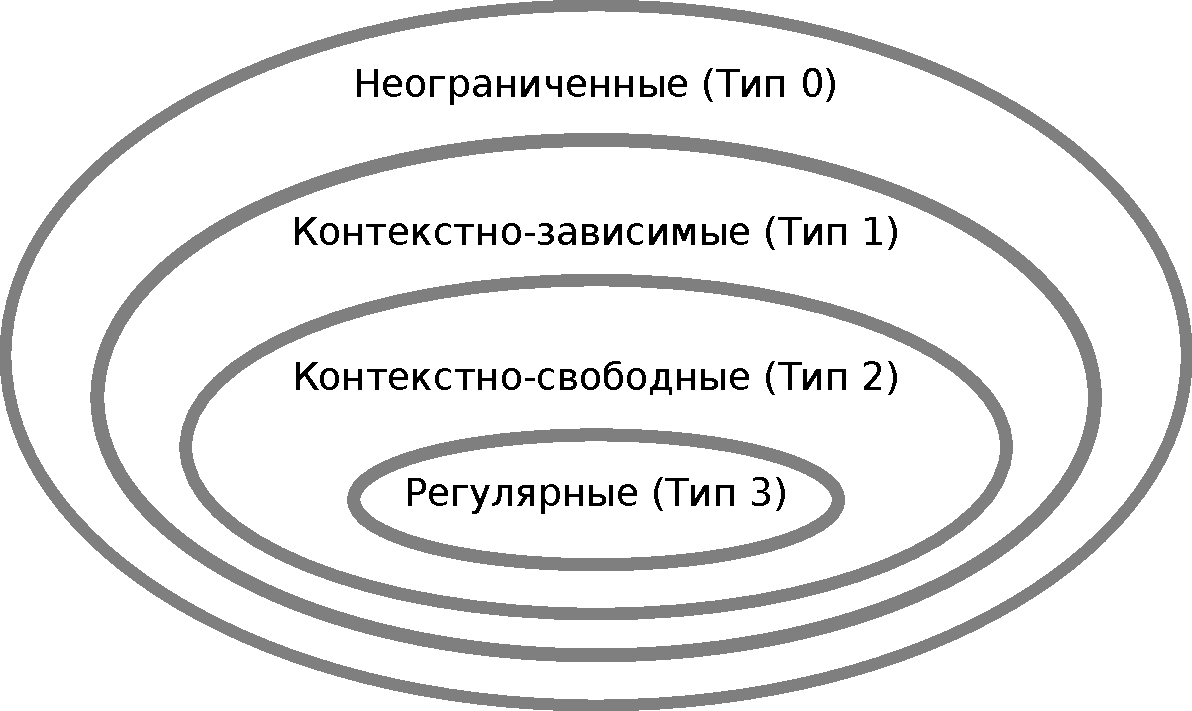
\includegraphics[width=0.9\textwidth]{figures/Chomsky.pdf}
  \end{center}
  \caption{Иерархия языков по Хомскому}
  \label{fig:Chomsky}
\end{figure}

Однако, данная иерархия постепенно теряет свою актуальность, так как появляются новые классы языков, свойства которых уже не удаётся адекватным образом отобразить, используя её.

Один из вариантов иерархии языков, более полно отображающий современное состояние дел, предложен Александром Охотиным\sidenote{Иерархия и некоторые отражаемые ей свойства подробно обсуждаются в презентации Александра Охотина ``Underlying principles
  and recurring ideas of formal grammars'' (\url{https://users.math-cs.spbu.ru/~okhotin/talks/grammars_lata_talk.pdf}).
  Также, с данной презентацией рекомендуется ознакомиться чтобы представить себе состояние области в целом.}.
Вариация предложенной Александром Охотиным иерархии представлена на изображении~\ref{fig:hierarchyOkhotin}~\sidenote{Данная вариация скомпонована из версии, представленной в презентации ``Underlying principles
  and recurring ideas of formal grammars'' и версии, взятой из работы~\cite{MRYKHIN2023113829}.}.
Представленная диаграмма содержит регулярные и контекстно-свободные.
Так и подклассы, лежащие между ними.
Вместе с этим, классы, лежащие выше контекстно-свободных: многокомпонентные контекстно-свободные, булевы, конъюнктивные, их подклассы.

\begin{figure*}
  \begin{center}
    \begin{tikzpicture}[node distance=1.0cm,bend angle=45,auto]
      \tikzstyle{lang}=[circle,thick,draw=blue!75,fill=blue!75,minimum size=1mm]
      \node [lang] (reg) [label=below:\textit{Reg}] {};
      \node [right of = reg] (reg_dummy) {};
      \node [lang] (lllin) [right of=reg_dummy, label=below:\textit{LLLin}] {};
      \node [right of = lllin] (lllin_dummy) {};
      \node [lang] (lrlin) [right of=lllin_dummy, label=below:\textit{LRLin}] {};
      \node [right of = lrlin] (lrlin_dummy) {};
      \node [lang] (unamblin) [right of=lrlin_dummy, label=below:\textit{UnambLin}] {};
      \node [right of = unamblin] (unamblin_dummy) {};
      \node [lang] (lin) [right of=unamblin_dummy, label=below:\textit{Lin}] {};
      \node [right of = lin] (lin_dummy) {};
      \node [right of = lin_dummy] (lin_dummy_2) {};
      \node [right of = lin_dummy_2] (lin_dummy_3) {};
      \node [lang] (conj) [right of=lin_dummy_3, label=below:\textit{Conj}] {};
      \node [right of = conj] (conj_dummy) {};
      \node [lang] (bool) [right of=conj_dummy, label=right:\textit{Bool}] {};
      
      \node [above of = lrlin] (lrlin_up_dummy) {};
      \node [lang] (ll) [above of=lrlin_up_dummy, label=above:\textit{LL}] {};
      \node [right of = ll] (ll_dummy) {};
      \node [lang] (lr) [right of=ll_dummy, label=above:\textit{LR}] {};
      \node [right of = lr] (lr_dummy) {};
      \node [lang] (unamb) [right of=lr_dummy, label=above:\textit{Unamb}] {};
      \node [right of = unamb] (unamb_dummy) {};
      \node [lang] (ordinary) [right of=unamb_dummy, label=right:\textit{Ordinary}] {};
      
      \node [lang] (conjleftcontext) [above of=conj_dummy, label=right:\textit{Conj$+\lhd$}] {};
      
      \node [below of = lrlin] (lrlin_down_dummy) {};
      \node [lang] (vpda) [below of=lrlin_down_dummy, label=below:\textit{VPDA}] {};
      \node [below of = lin] (lin_down_dummy_1) {};
      \node [below of = lin_down_dummy_1] (lin_down_dummy_2) {};
      \node [right of = lin_down_dummy_2] (lin_right_dummy_1) {};
      \node [lang] (linconj) [right of=lin_right_dummy_1, label=below:\textit{LinConj}] {};
      
      \node [lang] (unambtag) [above of=unamb_dummy, label=above:\textit{UnambTAG}] {};
      \node [right of = unambtag] (unambtag_dummy) {};
      \node [lang] (tag) [right of=unambtag_dummy, label=above:\textit{TAG}] {};
      \node [right of = tag] (tag_dummy) {};
      \node [lang] (mcfl) [right of=tag_dummy, label=above:\textit{MCFL}] {};
      
      \node [above of = linconj] (linconj_above_dummy) {};
      \node [lang] (unambconj) [right of=linconj_above_dummy, label=below:\textit{UnambConj}] {};
      \node [right of = unambconj] (unambconj_dummy) {};
      \node [lang] (unambbool) [right of=unambconj_dummy, label=right:\textit{UnambBool}] {};
      
      \node [below of = linconj] (linconj_below_dummy) {};
      \node [lang] (rtca) [right of=linconj_below_dummy, label=below:\textit{RT-CA}] {};
      \node [right of = rtca] (rtca_dummy) {};
      \node [lang] (ltca) [right of=rtca_dummy, label=right:\textit{LT-CA}] {};
      
      \path[->]
      (reg) edge node {} (lllin)
      (lllin) edge node {} (lrlin)
      (lrlin) edge node {} (unamblin)
      (unamblin) edge node {} (lin)
      
      (lllin) edge node {} (ll)
      (ll) edge node {} (lr)
      (ll) edge node {} (lr)
      (lr) edge node {} (unamb)
      (unamb) edge node {} (ordinary)
      
      (lrlin) edge node {} (lr)
      (unamblin) edge node {} (unamb)
      (lin) edge node {} (ordinary)
      
      (reg) edge node {} (vpda)
      (vpda) edge node {} (lr)
      (vpda) edge node {} (linconj)
      
      (ordinary) edge node {} (conj)
      (conj) edge node {} (bool)
      (conj) edge node {} (conjleftcontext)
      
      (unamb) edge node {} (unambtag)
      (ordinary) edge node {} (tag)
      (unambtag) edge node {} (tag)
      (tag) edge node {} (mcfl)
      
      (lin) edge node {} (linconj)
      (linconj) edge node {} (unambconj)
      (unambconj) edge node {} (unambbool)
      (unambconj) edge node {} (conj)
      (unambbool) edge node {} (bool)
      (unamb) edge node {} (unambconj)
      
      (linconj) edge node {} (rtca)
      (rtca) edge node {} (ltca)
      ;
    \end{tikzpicture}
  \end{center}
  \caption{Иерархия. \textit{Reg} --- регулярные, \textit{LLLin}, \textit{LRLin}, \textit{UnambLin}, \textit{Lin}, \textit{LL}, \textit{LR}, \textit{Unamb} --- однозначные, \textit{Ordinary} --- обыкновенные (контекстно-свободные)
    \textit{Conj}, \textit{Boolean}, \textit{UnamnbBool}, \textit{UnambConj}, \textit{VPDA}, \textit{LinConj}, \textit{UnambTAG}, \textit{TAG}, \textit{MCFL},}
  \label{fig:hierarchyOkhotin}
\end{figure*}

Для того, чтобы содержательно рассуждать про различные классы языков, необходимо иметь механизм, позволяющий чётко отделить один класс от другого.
\textit{Лемма о накачке} для соответствующего класса --- один из классических таких механизмов.
Однако, не для всех классов языков соответствующие результаты получены.
Так, например, формулировка леммы о накачки для многокомпонентных контекстно-свободных языков в общем виде всё ещё не найдена, хотя существуют формулировки для отдельных подклассов.
Аналогично, для булевых и конъюнктивных языков всё ещё не предложены аналоги лемм о накачке.


%\section{Вопросы и задачи}
%\begin{enumerate}
%  \item !!!
%  \item !!!
%\end{enumerate}


\backmatter
\setchapterstyle{plain}

\printbibliography

\end{document}
